\documentclass[12pt,a4paper]{article}
\usepackage{a4wide}
\usepackage[utf8]{inputenc}
\usepackage[T2A]{fontenc}
\usepackage{graphics,graphicx,epsfig}
\usepackage{amssymb,amsfonts,amsthm,amsmath,mathtext,cite,enumerate,float}
\usepackage[english,russian]{babel}
\usepackage[all]{xy}
\usepackage{morefloats}
\usepackage{pgf}
\usepackage[debug,outputdir={docgraphs/}]{dot2texi}
\usepackage{tikz}
\usepackage{scalefnt}
\usepackage{listings}
\usepackage{float}
\usepackage{verbatim}
\usepackage{placeins}
\usepackage{url}
\usepackage{babelbib}
\usepackage{pbox}
\usepackage{grffile}
\usepackage{color}
\usepackage{xfrac}
\usetikzlibrary{shapes,arrows}
\usetikzlibrary{decorations.pathmorphing}

% Comment the following block when compiling this .tex with a saner compiler than texlive.
\makeatletter
\def\@settitle{\begin{center}%
    \baselineskip14\p@\relax
    \bfseries
    \@title
  \end{center}%
}

%\renewcommand{\section}{\@startsection {section}{1}%
%  \z@{.7\linespacing\@plus\linespacing}{.5\linespacing}%
%  {\normalfont}}
%\renewcommand{\section}{\@startsection {section}{1}
%  \z@{2.7ex \@plus 1ex}{1.0ex}%
%  {\normalfont}}
\makeatother

\newtheorem{algo}{Алгоритм}
\newtheorem{theorem}{Теорема}
\newtheorem{stat}{Утверждение}
\newtheorem{defin}{Определение}

\begin{document}
% Comment the following block when compiling this .tex with a saner compiler than texlive.
\lstset{language=C++}

\begin{center}
  ВОССТАНОВЛЕНИЕ ДИСПЕРСИИ ПРОЗРАЧНОЙ СРЕДЫ ПО ЭКСПЕРИМЕНТАЛЬНЫМ ДАННЫМ

  \bigskip
  Г.\,И.~Рудой
\end{center}

\begin{abstract}
  Для восстановления нелинейной зависимости показателя преломления среды от длины
  волны рассматривается набор индуктивно порожденных моделей с целью выбора оптимальной.
  Применяется алгоритм индуктивного порождения допустимых существенно
  нелинейных моделей. Предлагается метод оценки устойчивости полученного решения.
  Приводятся результаты численного моделирования на данных, полученных в ходе
  эксперимента по определению состава смеси по ммарной дисперсии.

  \bigskip
  \textbf{Ключевые слова}: \emph{символьная регрессия, нелинейные модели, индуктивное порождение,
	стабильность решений, дисперсия прозрачной среды.}
\end{abstract}

\section*{Введение}

В ряде прикладных областей возникает задача восстановления зависимости показателя
преломления прозрачной для света среды от длины волны. И задаваемая в ходе эксперимента
длина волны, и измеряемый коэффициент преломления, соответствующий этой длине волны,
определяются с достаточно высокой точностью в широком диапазоне длин волн.

\textcolor{red}{TODO описать вкратце ход эксперимента.}

Физические соображения \cite{Sivukhin05,Serova11} определяют некоторый общий вид
зависимости коэффициента преломления прозрачной среды от длины волны, которой должны
описываться экспериментальные данные. Для эксперта представляют интерес конкретные
параметры этой зависимости, поэтому требуется экспертная интерпретация полученной
модели.

Кроме того, каждое измерение имеет свою допустимую погрешность, задаваемую
экспериментатором \textcolor{red}{TODO попробовать сослаться на методику оценки погрешности в подобных экспериментах}, поэтому необходимо оценить устойчивость полученных результатов.
Иными словами, требуется понять, насколько сильно меняются коэффициенты
результирующей суперпозиции с фиксированной структурой
при небольшом изменении экспериментальных данных.

В настоящей работе исследуется возможность применения алгоритма, предложенного в
\cite{Rudoy13} для восстановления искомой зависимости, и результаты его работы
сравниваются с результатами применения SVM-регрессии. Кроме того, исследуется
влияние штрафа за сложность на качество и структурную сложность получающихся
суперпозиций. Также исследуется возможность оценки устойчивости решения и вклада
различных элементов результирующей модели.

В первой части данной работы формально поставлена задача восстановления
дисперсии жидкости. Во второй части вкратце описывается алгоритм \cite{Rudoy13},
используемый для порождения аналитической функции-суперпозиции, аппроксимирующей
данные. В третьей части описывается метод, позволяющий учитывать и анализировать
вклад различных членов порожденной суперпозици и их зависимость от погрешности
эксперимента. В четвертой части приводятся результаты вычислительного
эксперимента на реальных данных, полученных в ходе физического эксперимента по
изучению возможности определения состава смеси прозрачных веществ по
суммарной дисперсионной зависимости. Рассматривается три прозрачных для света
вещества, для каждого из которых имеется 18 экспериментальных точек,
соответствующих величине коэффициента преломления при различных значениях длины волны.

\section{Постановка задачи}

Дана выборка $\tilde{D}$ из $\ell$ результатов измерений коэффициента преломления для некоторого
вещества: $\tilde{D} = \{ \tilde{\lambda}_i, \tilde{n}_i \}$, где $\tilde{\lambda}_i$~--- длина волны,
а $\tilde{n}_i$~--- измеренный коэффициент преломления в $i$-ом измерении.

Требуется найти функцию $\hat{f} = \hat{f}(\lambda)$, минимизирующую функционал
потерь в предположении о нормальности случайной ошибки эксперимента:
\begin{equation}
  S(f, D) = \sum_{i = 1}^\ell (f(\lambda_i) - n_i)^2 \rightarrow \min_{f \in \mathcal{F}},
  \label{eq:s}
\end{equation}
где $D = \{ \lambda_i, n_i \mid i \in \{ 1, \dots, \ell \} \}$, а $\mathcal{F}$~---
некоторое множество суперпозиций, из которого выбирается оптимальная.

Иными словами,
\begin{equation}
  \hat{f}(\lambda) = \hat{f}_D(\lambda) = \mathop{\arg \min}\limits_{f \in \mathcal{F}} S(f, D).
  \label{eq:fhat}
\end{equation}

Введем понятие устойчивости суперпозиции $f$. Рассмотрим вектор параметров
$\boldsymbol{\omega}_f = \{ \omega_i^f \mid i \in \{ 1, \dots, l_f \} \} $ суперпозиции $f$: $f(\lambda) = f(\lambda, \boldsymbol{\omega}_f)$.
Пусть для некоторой выборки $D = \{ \lambda_i, n_i \}$ функция $f_D$ с
вектором параметров $\hat{\boldsymbol{\omega}}_{f_D}$ минимизирует
функционал \eqref{eq:s}. Рассмотрим выборку
\begin{equation}
  \acute{D}(\sigma_n, \sigma_{\lambda}) = \{ \lambda_i + \xi^{\lambda}_i, n + \xi^n_i \mid i \in 1, \dots, \ell; \xi^n_i \in \mathcal{N}(0, \sigma_n); \xi^{\lambda}_i \in \mathcal{N}(0, \sigma_{\lambda}) \}.
  \label{eq:d_acute}
\end{equation}
Для этой выборки найдем оптимальный вектор $\acute{\hat{\boldsymbol{\omega}}}_{f_D, \sigma_n, \sigma_{\lambda}}$
параметров суперпозиции $f_D$, минимизирующий функционал \eqref{eq:s}:
\begin{equation}
  \acute{\hat{\boldsymbol{\omega}}}_{f_D, \sigma_n, \sigma_{\lambda}} = \mathop{\arg \min}\limits_{\boldsymbol{\omega}_{f_D} \in R^{\mid \hat{\boldsymbol{\omega}}_{f_D} \mid}} S (f_D (\cdot, \boldsymbol{\omega}_{f_D}), \acute{D}).
  \label{eq:hat_omega}
\end{equation}
Понятно, что $\acute{\hat{\boldsymbol{\omega}}}_{f_D, \sigma_n, \sigma_{\lambda}}$~---
векторная случайная величина, и, следовательно,
$\hat{\boldsymbol{\omega}}_{f_D} - \acute{\hat{\boldsymbol{\omega}}}_{f_D, \sigma_n, \sigma_{\lambda}}$~---
также векторная случайная величина.

Пусть дан набор выборок $\acute{\mathcal{D}}_N = \{ \acute{D}_1, \dots, \acute{D}_N \}$, и пусть
$\overline{\sigma}_i$~--- эмпирическое стандартное отклонение $i$-ой компоненты
векторной случайной величины
$\hat{\boldsymbol{\omega}}_{f_D} - \acute{\hat{\boldsymbol{\omega}}}_{f_D, \sigma_n, \sigma_{\lambda}}$
на множестве $\acute{\mathcal{D}}_N$.
\emph{Относительной устойчивостью} (или просто \emph{устойчивостью}) параметра
$\omega_i$ относительно вектора $\boldsymbol{\alpha}$ будем называть вектор
\begin{equation}
  \mathbf{T}_f^{\boldsymbol{\alpha}}(i) = \big\{ \frac{\frac{\overline{\sigma}_i}{\hat{\omega}_i}}{\frac{\sigma_{\alpha_j}}{\alpha_j}} \big\}.
  \label{eq:t_rel}
\end{equation}
В частности, в искомой задаче восстановления дисперсионной зависимости,
\[
  \mathbf{T}_f^{\{ n, \lambda \}}(i) = \big\{ \frac{\frac{\overline{\sigma}_i}{\hat{\omega}_i}}{\frac{\sigma_n}{n}}, \frac{\frac{\overline{\sigma}_i}{\hat{\omega}_i}}{\frac{\sigma_{\lambda}}{\lambda}} \big\}.
\]

Матрицу, столбцами которой являются векторы $\mathbf{T}_f^{\boldsymbol{\alpha}}(i) \mid i \in \{ 1, \dots, l_f \}$,
будем называть устойчивостью функции $f$ относительно вектора $\boldsymbol{\alpha}$
и обозначать $\mathbb{T}_f^{\boldsymbol{\alpha}}$.

Требуется исследовать зависимость устойчивости $\mathbb{T}_{\hat{f}}^{\{ n, \lambda \}}$ относительно
вектора $\{ n, \lambda \}$ от $\sigma_n$ и $\sigma_{\lambda}$. В дальнейшем там,
где это не приведет к неоднозначностям, $\mathbb{T}_{\hat{f}}^{\{ n, \lambda \}}$
будет обозначаться как $\mathbb{T}_f$,

Кроме того, отдельный интерес представляет и вектор первых производных
устойчивости $\mathbb{T}_f^{\boldsymbol{\alpha}}$ по $\boldsymbol{\alpha}$:
\[
  \frac{\partial \mathbb{T}_f^{\boldsymbol{\alpha}}}{\partial{\boldsymbol{\alpha}}},
\]
являющийся характеристикой изменения устойчивости $\mathbb{T}$ при изменении
стандартных отклонений погрешностей, накладываемых на обучающую выборку.

\section{Алгоритм индуктивного порождения суперпозиций}

Опишем предложенный в \cite{Rudoy13} алгоритм.

Пусть задано некоторое множество $G = \{ g_1, \dots, g_k \}$ 
порождающих функций. Набор суперпозиций $\mathcal{F} = \{ f \}$
инициализируется случайными суперпозициями функций $g \in G$. Суперпозиции из
$\mathcal{F}$ содержат как свободные переменные, соответствующие
компонентам вектора-описания объектов из генеральной совокупности, так и
константы, которые оптимизируются на каждом шаге алгоритмом Левенберга-Марквардта
согласно введенному функционалу потерь \eqref{eq:s}. Также на каждой итерации
над суперпозициями выполняется набор модифицирующих операций с целью улучшения
качества $Q_f$ суперпозиций.

Качество $Q_f$ суперпозиции $f$ вычисляется по совокупности точности приближения
экспериментальных данных и структурной сложности суперпозиции по следующей формуле:
\begin{equation}
  Q_f = \frac{1}{1 + S(f)} \left(\alpha + \frac{1 - \alpha}{1 + \text{exp} (C_f - \tau)}\right),
  \label{eq:s_f}
\end{equation}
где:
\begin{itemize}
  \item[] $S(f)$~--- значение функционала потерь \eqref{eq:s} на данной выборке $D$;
  \item[] $C_f$~--- сложность суперпозиции, соответствующая количеству элементарных
	функций, свободных переменных и констант;
  \item[] $\alpha$~--- $0 \ll \alpha < 1$, характеризует влияние штрафа за сложность
	на качество суперпозиции (большие значения $\alpha$ отдают предпочтение более
	точным моделям, а меньшие~--- более простым);
  \item[] $\tau$~--- коэффициент, характеризующий желаемую сложность модели.
\end{itemize}

Второй множитель в \eqref{eq:s_f} выполняет роль штрафа за слишком
большую сложность суперпозиции, что подавляет эффект переобучения и позволяет
получать более простые суперпозиции ценой большей ошибки на обучающих данных
при большей обобщающей способности.

Отметим, что параметры $\alpha$ и $\tau$ выбираются экспертом.

Таким образом, исходная задача минимизации функционала \eqref{eq:s} заменяется
на задачу минимизации функционала \eqref{eq:s_f}:
\begin{equation}
  Q_f = \frac{1}{1 + S(f)} \left(\alpha + \frac{1 - \alpha}{1 + \text{exp} (C_f - \tau)}\right) \rightarrow \min_{f \in \mathcal{F}}.
  \label{eq:s_f_min}
\end{equation}

\section{Метод исследования стабильности решения}

Для оценки устойчивости $\mathbb{T}_{\hat{f}}$ решения $\hat{f}$ задачи
\eqref{eq:s_f} предлагается следующий подход. Фиксируется структурный вид суперпозиции
$\hat{f}$, и исследуется зависимость стандартного отклонения ее коэффициентов
как функция стандартного отклонения нормально распределенной случайной добавки
в исходных данных.

Иными словами, выбираются значения $\sigma_{\lambda}$ и $\sigma_n$, затем для этих
значений генерируется выборка $\acute{D}(\sigma_n, \sigma_{\lambda})$ согласно
\eqref{eq:d_acute}. Для этой выборки вычисляются значения коэффициентов суперпозиции
$\hat{f}$, минимизирующие функционал \eqref{eq:s} согласно \eqref{eq:hat_omega},
методом Левенберга-Марквардта.

Данная процедура для фиксированной пары $\sigma_{\lambda}$ и $\sigma_n$ повторяется
до достижения некоторого критерия останова (например, по количеству итераций),
после которого и рассчитывается $\mathbb{T}_{\hat{f}}$.

Повторяя описанные выше шаги для различных $\sigma_{\lambda}$ и $\sigma_n$, можно
оценить зависимость стандартного отклонения коэффициентов суперпозиции от
стандартного отклонения шума.

Из физических соображений ясно, что гладкая зависимость означает устойчивое в
физическом смысле решение, тогда как отклонения от гладкости означают
ту или иную ошибку в суперпозиции и могут являться свидетельством переобучения.

Кроме того, сравнение различных суперпозиций может также производиться по
критерию устойчивости в дополнение к сравнению по сложности и по значению
функционала \eqref{eq:s}.

\section{Вычислительный эксперимент}

В вычислительном эксперименте используются данные, полученные в ходе
изучения возможности определения состава смеси прозрачных
веществ по суммарной дисперсионной зависимости, если известна экспериментальная
зависимость дисперсии для каждого конкретного веществ. Рассматривается три
вещества, для каждого из которых имеется 18 экспериментальных точек,
соответствующих коэффициенту преломления при разных значениях длины волны.
Значения приведены в таблице \ref{tabl:source_data}.

\begin{table}[h]
  \begin{tabular}{| r | r | r | r |} \hline
	$\lambda$, нм	& Первый материал & Второй материал & Третий материал \\ \hline
	435.8 & 1.36852 & 1.35715 & 1.34850 \\ \hline
	447.1 & 1.36745 & 1.35625 & 1.34767 \\ \hline
	471.3 & 1.36543 & 1.35449 & 1.34620 \\ \hline
	486.1 & 1.36446 & 1.35349 & 1.34542 \\ \hline
	501.6 & 1.36347 & 1.35275 & 1.34461 \\ \hline
	546.1 & 1.36126 & 1.35083 & 1.34294 \\ \hline
	577.0 & 1.3599 & 1.34968 & 1.34191 \\ \hline
	587.6 & 1.3597 & 1.34946 & 1.34174 \\ \hline
	589.3 & 1.35952 & 1.34938 & 1.34158 \\ \hline
	656.3 & 1.35767 & 1.34768 & 1.34005 \\ \hline
	667.8 & 1.35743 & 1.34740 & 1.33987 \\ \hline
	706.5 & 1.35652 & 1.34664 & 1.33917 \\ \hline
	750 & 1.35587 & 1.34607 & 1.33855 \\ \hline
	800 & 1.35504 & 1.34544 & 1.33794 \\ \hline
	850 & 1.3544 & 1.34487 & 1.33741 \\ \hline
	900 & 1.35403 & 1.34437 & 1.33685 \\ \hline
	950 & 1.35364 & 1.34407 & 1.33652 \\ \hline
  \end{tabular}
  \caption{Экспериментальные значения коэффициентов преломления для трех разных материалов.}
  \label{tabl:source_data}
\end{table}

Предполагается, что дисперсионные свойства веществ описываются одной и той же функциональной зависимостью, так
как подчиняются одним и тем же законам. Поэтому сначала получена суперпозиция $\hat{f}$,
минимиризующая \eqref{eq:s_f} для первого вещества, а затем для каждого
из трех веществ находятся соответствующие векторы параметров
$\hat{\boldsymbol{\omega}}_{\hat{f}}$ и оценивается устойчивость полученного решения.

Разделение на обучающую и контрольную выборку не производилось, однако переобучения
удается избежать и без такого разделения, опираясь целиком на штраф за сложность.

Из физических соображений следует \cite{Serova11}, что зависимость коэффициента
преломления $n$ от длины волны $\lambda$ должна выражаться суммой отрицательных
четных степеней дисперсии, поэтому множество элементарных функций состоит из
стандартных операций сложения и умножения:
\[
  g_1(x_1, x_2) = x_1 + x_2,
\]
\[
  g_2(x_1, x_2) = x_1 x_2,
\]
а также из функции
\[
  g_3(\lambda, p) = \frac{1}{\lambda^{2p}}.
\]

В ходе вычислительного эксперимента константы, меньшие $10^{-7}$,
заменялись на $0$.

В результате применения описанного выше алгоритма со значениями
$\alpha = 0.05$, $\tau = 10$ получена следующая суперпозиция
(константы округлены до третьей значащей цифры для удобства чтения):
\begin{equation}
  f(\lambda) = 1.35 + \frac{5.82}{\lambda^2} + \frac{3.58 \cdot 10^{-5}}{\lambda^4},
  \label{eq:res_0}
\end{equation}
со сложностью $13$, среднеквадратичной ошибкой $2.2 \cdot 10^{-5}$ и значением $Q_f \approx 0.0475$.

Отметим, что обычно в приложениях учитывают только квадратичный член, а более
высокими степенями пренебрегают. Коэффициент при $\frac{1}{\lambda^4}$ указывает
на полное согласие полученных результатов с принятой практикой.

\paragraph{Влияние штрафа за сложность.}

Исследуем, как влияет добавление нечетных степеней на результат решения задачи \eqref{eq:s_f_min},
заменив функцию $g_3$ в порождающем наборе на
\[
  g_3(\lambda, p) = \frac{1}{\lambda^p}.
\]

Следует отметить, что при тех же $\alpha = 0.05$ и $\tau = 10$ результирующей функцией остается
\eqref{eq:res_0}.

Увеличим $\tau$ до 25. Получим следующую формулу:
\begin{equation}
  n(\lambda) = 1.34 + \frac{11.6}{\lambda} + \frac{17.37}{\lambda^2} + \frac{0.0866}{\lambda^3} + \frac{2.95 \cdot 10^{-4}}{\lambda^4} + \frac{8.54 \cdot 10^{-7}}{\lambda^5},
  \label{eq:res_incorrect}
\end{equation}
сложность которой составляет $31$, и для которой среднеквадратичная ошибка
на выборке составляет $\approx 3.9 \cdot 10^{-7}$,
а значение $Q_f \approx 0.0498$.

Иными словами, при большей желаемой сложности,
регулируемой параметром $\tau$, выигрывает более сложная (а в данном случае и
физически некорректная) модель, которая лучше описывает экспериментальные данные.

То есть, как и следовало ожидать, чрезмерное увеличение $\tau$ ведет к переобучению.

\paragraph{SVM.}

В качестве базового алгоритма используется SVM-регрессия с RBF-ядром \cite{Vapnik79}.
Параметр $\gamma$ ядра подбирался по методу скользящего контроля, наилучшим результатом является
комбинация из $15$ опорных векторов c $\gamma \approx 2 \cdot 10^{-6}$, при этом
среднеквадратичная ошибка при кросс-валидации с тестовой выборкой, содержащей по 2
объекта, составляет $8.96 \cdot 10^{-8}$. Однако, проинтерпретировать полученную
решающую функцию не представляется возможным.

\paragraph{Исследование стабильности решения.}

Для оценки стабильности решения фиксировалась формула \eqref{eq:res_0} и исследовалась
зависимость стандартного отклонения ее коэффициентов от стандартного отклонения
нормально распределенного случайного шума в исходных данных описанным выше методом.
Критерием останова в нем являлось достижение 10000 итераций для каждой пары
$(\sigma_{\lambda}, \sigma_n)$.

Численные значения эмпирического матожидания и дисперсии для первого, второго и третьего
коэффициентов формулы \eqref{eq:res_0} для первого полимера для некоторых значений
$(\sigma_{\lambda}, \sigma_n)$ приведены в таблицах \ref{tabl:stability1},
\ref{tabl:stability2} и \ref{tabl:stability3} соответственно. По строкам указаны значения
для $\sigma_n$, по столбцам~--- для $\sigma_{\lambda}$.

\begin{table}[h]
  \centering
  \resizebox{\columnwidth}{!}{%
	\begin{tabular}{| l | l | l | l | l | l |} \hline
	   & $0$ & $10^{-5}$ & $10^{-4}$ & $0.001$ & $0.01$\\ \hline
	  0 & $\displaystyle (1.36; 5.97 \cdot 10^{-7})$ & $\displaystyle (1.36; 2.34 \cdot 10^{-6})$ & $\displaystyle (1.36; 2.39 \cdot 10^{-5})$ & $\displaystyle (1.36; 2.34 \cdot 10^{-4})$ & $\displaystyle (1.36; 0.00238)$\\ \hline
	  0.01 & $\displaystyle (1.36; 0)$ & $\displaystyle (1.36; 2.37 \cdot 10^{-6})$ & $\displaystyle (1.36; 2.38 \cdot 10^{-5})$ & $\displaystyle (1.36; 2.37 \cdot 10^{-4})$ & $\displaystyle (1.36; 0.00231)$\\ \hline
	  0.1 & $\displaystyle (1.36; 0)$ & $\displaystyle (1.36; 2.37 \cdot 10^{-6})$ & $\displaystyle (1.36; 2.35 \cdot 10^{-5})$ & $\displaystyle (1.36; 2.34 \cdot 10^{-4})$ & $\displaystyle (1.36; 0.00237)$\\ \hline
	  1 & $\displaystyle (1.36; 1.03 \cdot 10^{-7})$ & $\displaystyle (1.36; 2.36 \cdot 10^{-6})$ & $\displaystyle (1.36; 2.34 \cdot 10^{-5})$ & $\displaystyle (1.36; 2.39 \cdot 10^{-4})$ & $\displaystyle (1.36; 0.00235)$\\ \hline
	  10 & $\displaystyle (1.36; 2.74 \cdot 10^{-7})$ & $\displaystyle (1.36; 2.37 \cdot 10^{-6})$ & $\displaystyle (1.36; 2.35 \cdot 10^{-5})$ & $\displaystyle (1.36; 2.35 \cdot 10^{-4})$ & $\displaystyle (1.36; 0.00236)$\\ \hline
	\end{tabular}%
  }
  \caption{Значения матожидания и стандартного отклонения для первого коэффициента первого полимера}
  \label{tabl:stability1}
\end{table}

\begin{table}[h]
  \centering
  \resizebox{\columnwidth}{!}{%
	\begin{tabular}{| l | l | l | l | l | l |} \hline
	   & $0$ & $10^{-5}$ & $10^{-4}$ & $0.001$ & $0.01$\\ \hline
	  0 & $\displaystyle (5.82; 0)$ & $\displaystyle (5.82; 9.12 \cdot 10^{-4})$ & $\displaystyle (5.82; 0.00913)$ & $\displaystyle (5.82; 0.0871)$ & $\displaystyle (5.55; 1.87)$\\ \hline
	  0.01 & $\displaystyle (5.82; 5.41 \cdot 10^{-5})$ & $\displaystyle (5.82; 9.17 \cdot 10^{-4})$ & $\displaystyle (5.82; 0.00904)$ & $\displaystyle (5.82; 0.0867)$ & $\displaystyle (5.56; 1.81)$\\ \hline
	  0.1 & $\displaystyle (5.82; 5.37 \cdot 10^{-4})$ & $\displaystyle (5.82; 0.00105)$ & $\displaystyle (5.82; 0.00907)$ & $\displaystyle (5.82; 0.0873)$ & $\displaystyle (5.56; 1.81)$\\ \hline
	  1 & $\displaystyle (5.82; 0.00538)$ & $\displaystyle (5.82; 0.00549)$ & $\displaystyle (5.82; 0.0106)$ & $\displaystyle (5.82; 0.0866)$ & $\displaystyle (5.56; 1.82)$\\ \hline
	  10 & $\displaystyle (5.82; 0.0511)$ & $\displaystyle (5.82; 0.0516)$ & $\displaystyle (5.82; 0.0.20)$ & $\displaystyle (5.82; 0.103)$ & $\displaystyle (5.59; 1.75)$\\ \hline
	\end{tabular}%
  }
  \caption{Значения матожидания и стандартного отклонения для второго коэффициента первого полимера}
  \label{tabl:stability2}
\end{table}

\begin{table}[h]
  \centering
  \resizebox{\columnwidth}{!}{%
	\begin{tabular}{| l | l | l | l | l | l |} \hline
	   & $0$ & $10^{-5}$ & $10^{-4}$ & $0.001$ & $0.01$\\ \hline
	  0 & $\displaystyle (3.58 \cdot 10^{-5}; 0)$ & $\displaystyle (3.58 \cdot 10^{-5}; 0)$ & $\displaystyle (3.58 \cdot 10^{-5}; 0)$ & $\displaystyle (3.58 \cdot 10^{-5}; 6.21 \cdot 10^{-7})$ & $\displaystyle (0; 0.0657)$\\ \hline
	  0.01 & $\displaystyle (3.58 \cdot 10^{-5}; 0)$ & $\displaystyle (3.58 \cdot 10^{-5}; 0)$ & $\displaystyle (3.58 \cdot 10^{-5}; 0)$ & $\displaystyle (3.58 \cdot 10^{-5}; 6.23 \cdot 10^{-7})$ & $\displaystyle (5.7 \cdot 10^{-4}; 0.0536)$\\ \hline
	  0.1 & $\displaystyle (3.58 \cdot 10^{-5}; 0)$ & $\displaystyle (3.58 \cdot 10^{-5}; 0)$ & $\displaystyle (3.58 \cdot 10^{-5}; 0)$ & $\displaystyle (3.58 \cdot 10^{-5}; 6.21 \cdot 10^{-7})$ & $\displaystyle (0; 0.106)$\\ \hline
	  1 & $\displaystyle (3.58 \cdot 10^{-5}; 0)$ & $\displaystyle (3.58 \cdot 10^{-5}; 0)$ & $\displaystyle (3.58 \cdot 10^{-5}; 1.16 \cdot 10^{-7})$ & $\displaystyle (3.58 \cdot 10^{-5}; 6.32 \cdot 10^{-7})$ & $\displaystyle (0; 0.185)$\\ \hline
	  10 & $\displaystyle (3.59 \cdot 10^{-5}; 9.71 \cdot 10^{-7})$ & $\displaystyle (3.59 \cdot 10^{-5}; 9.83 \cdot 10^{-7})$ & $\displaystyle (3.59 \cdot 10^{-5}; 9.89 \cdot 10^{-7})$ & $\displaystyle (3.59 \cdot 10^{-5}; 1.18 \cdot 10^{-6})$ & $\displaystyle (2.4 \cdot 10^{-4}; 0.0882)$\\ \hline
	\end{tabular}%
  }
  \caption{Значения матожидания и стандартного отклонения для третьего коэффициента первого полимера}
  \label{tabl:stability3}
\end{table}

В таблице \ref{tabl:res_even} представлены
поверхности уровня дисперсии для первого, второго и третьего коэффициентов каждого из полимеров
соответственно.

\begin{table}[h]
  \centering
  \begin{tabular}{c c c}
	Материал 1 & Материал 2 & Материал 3 \\ \hline
	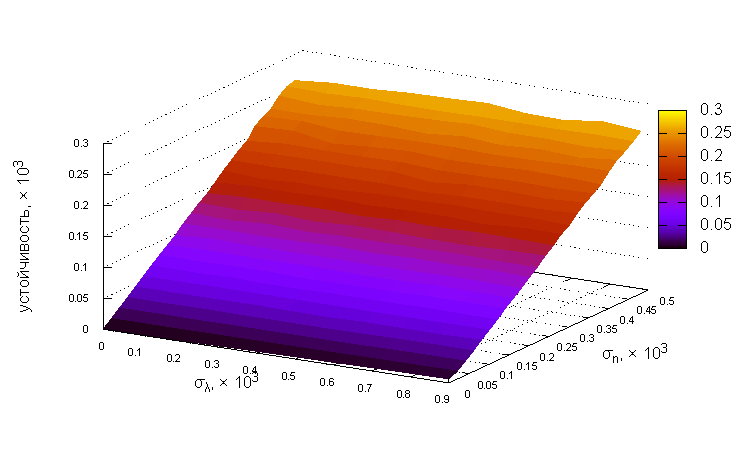
\includegraphics[scale=0.25]{figs/even/p1.txt_coeff0.dat.pdf} & 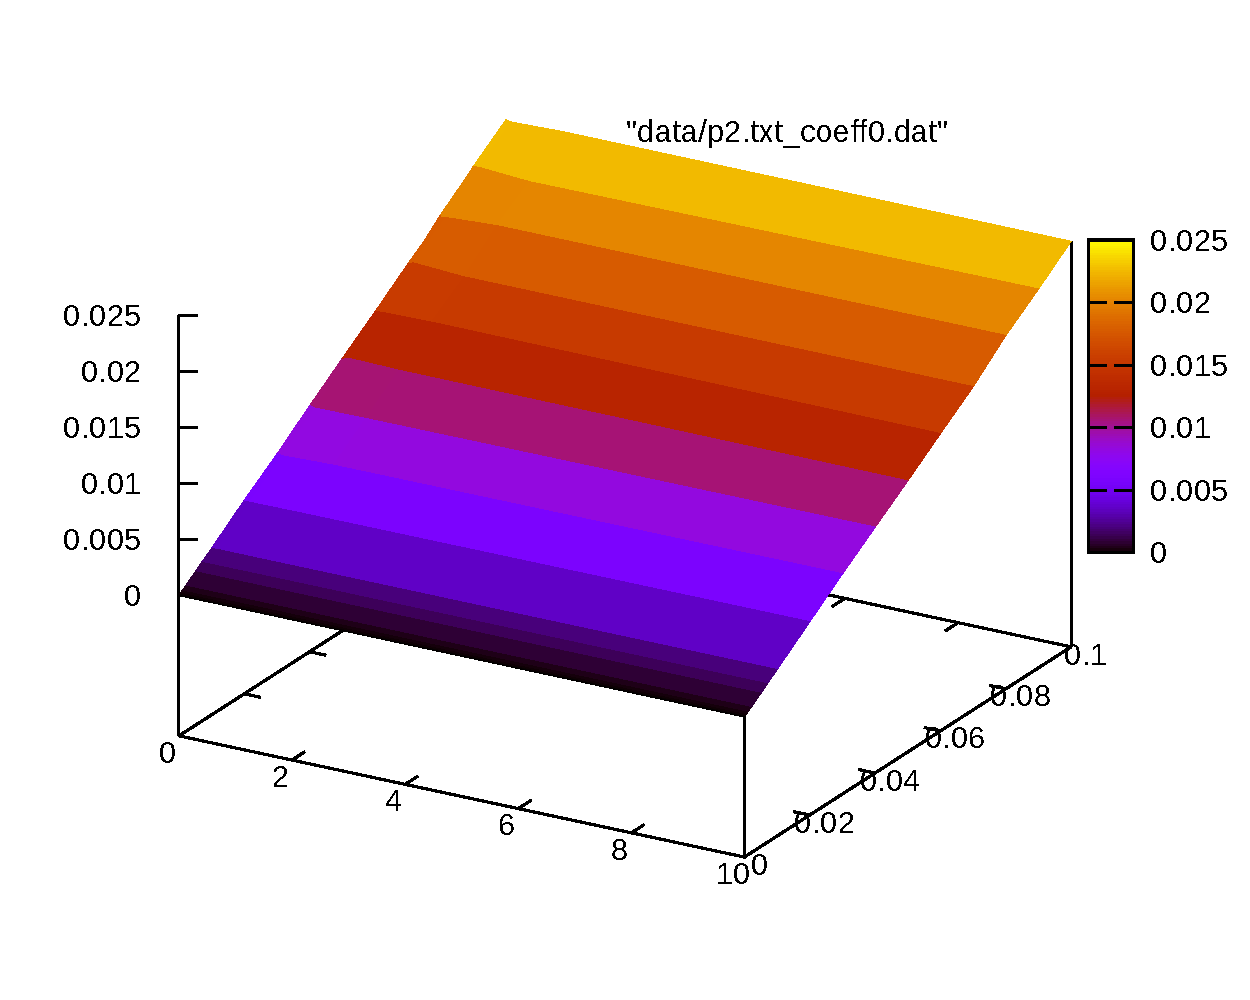
\includegraphics[scale=0.25]{figs/even/p2.txt_coeff0.dat.pdf} & 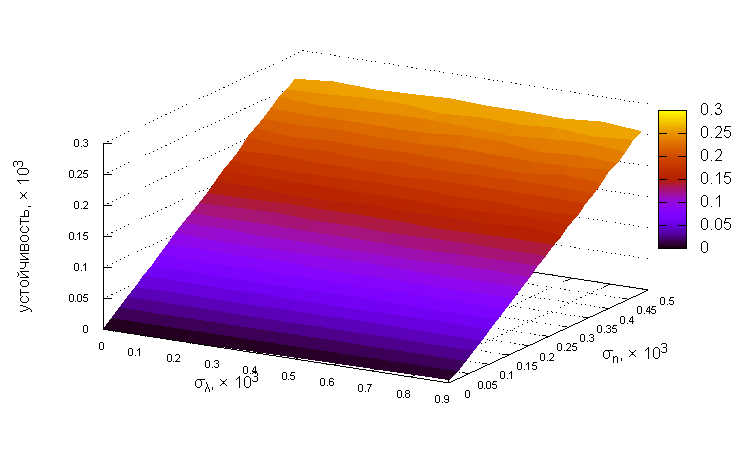
\includegraphics[scale=0.2]{figs/even/p3.txt_coeff0.dat.pdf} \\
	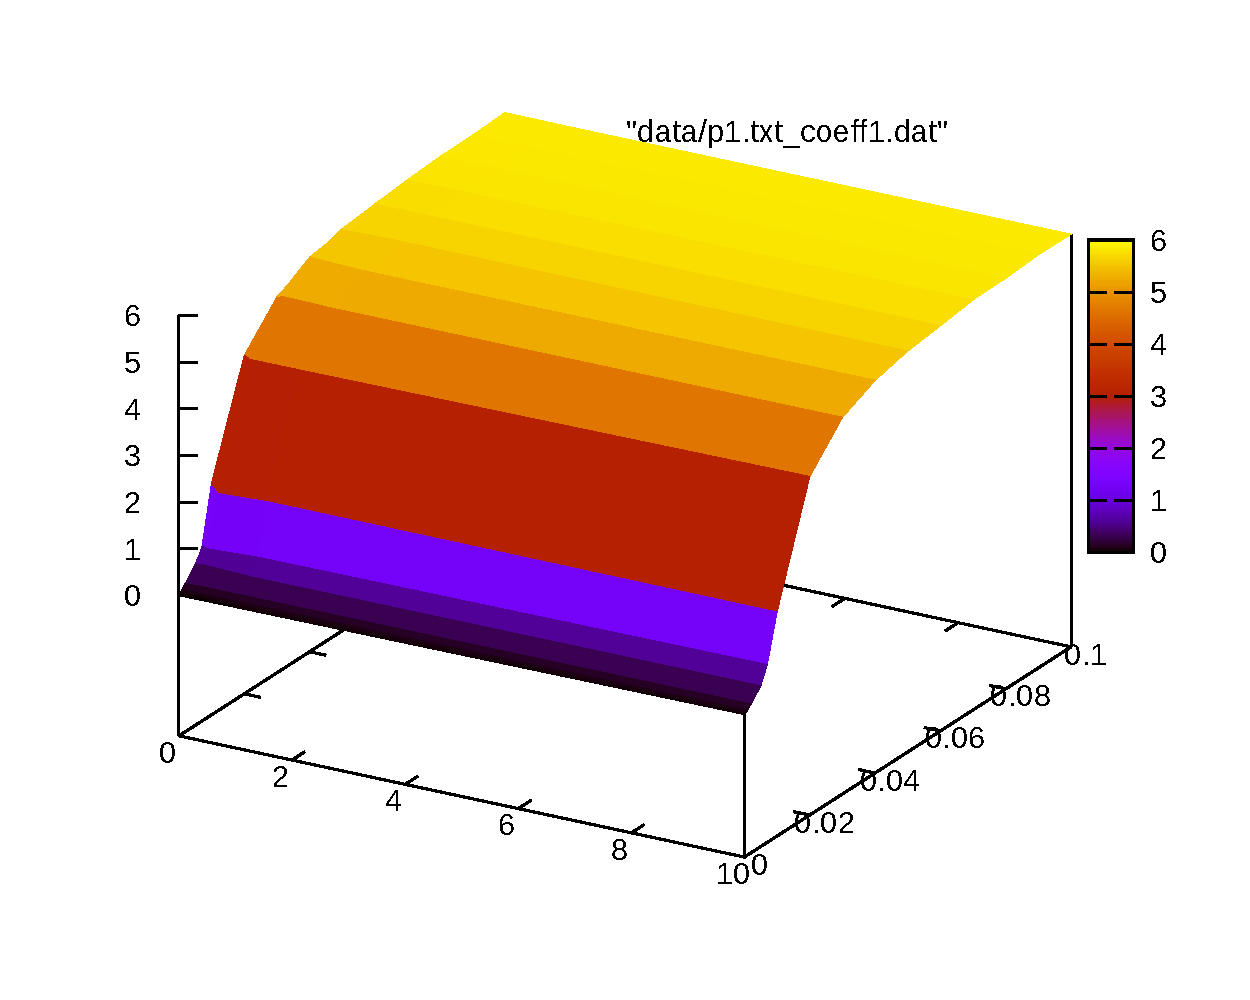
\includegraphics[scale=0.25]{figs/even/p1.txt_coeff1.dat.pdf} & 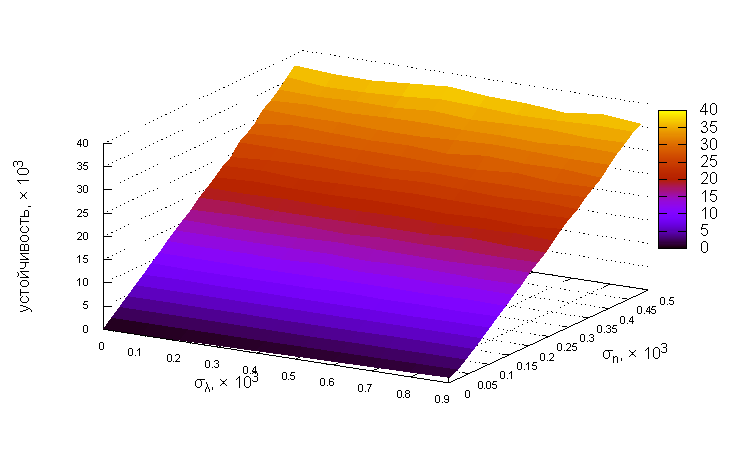
\includegraphics[scale=0.25]{figs/even/p2.txt_coeff1.dat.pdf} & 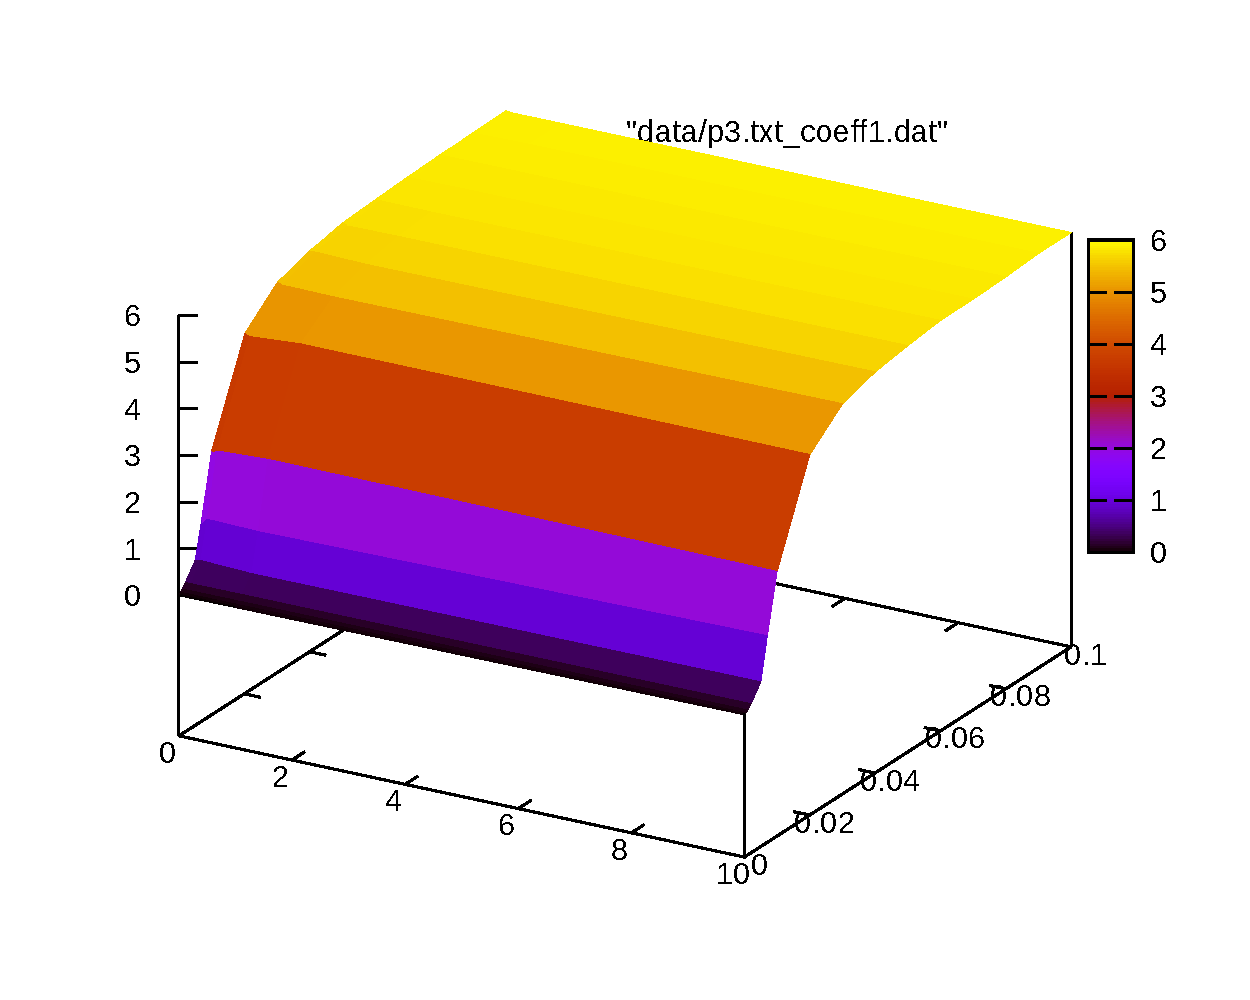
\includegraphics[scale=0.25]{figs/even/p3.txt_coeff1.dat.pdf} \\
	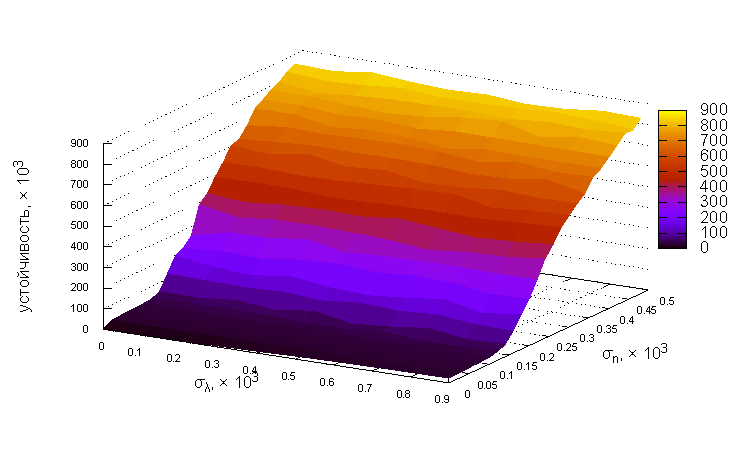
\includegraphics[scale=0.25]{figs/even/p1.txt_coeff2.dat.pdf} & 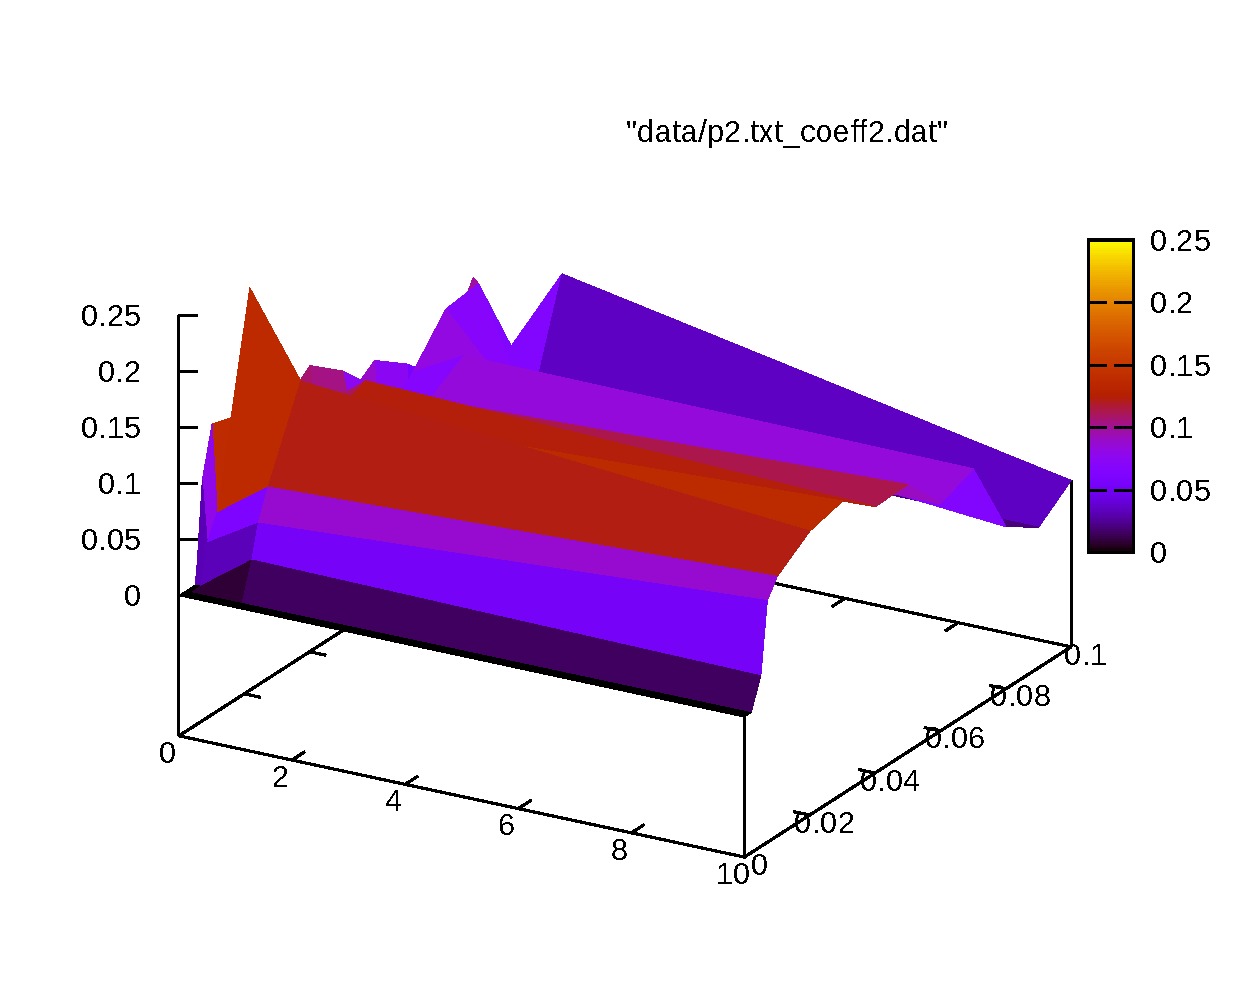
\includegraphics[scale=0.25]{figs/even/p2.txt_coeff2.dat.pdf} & 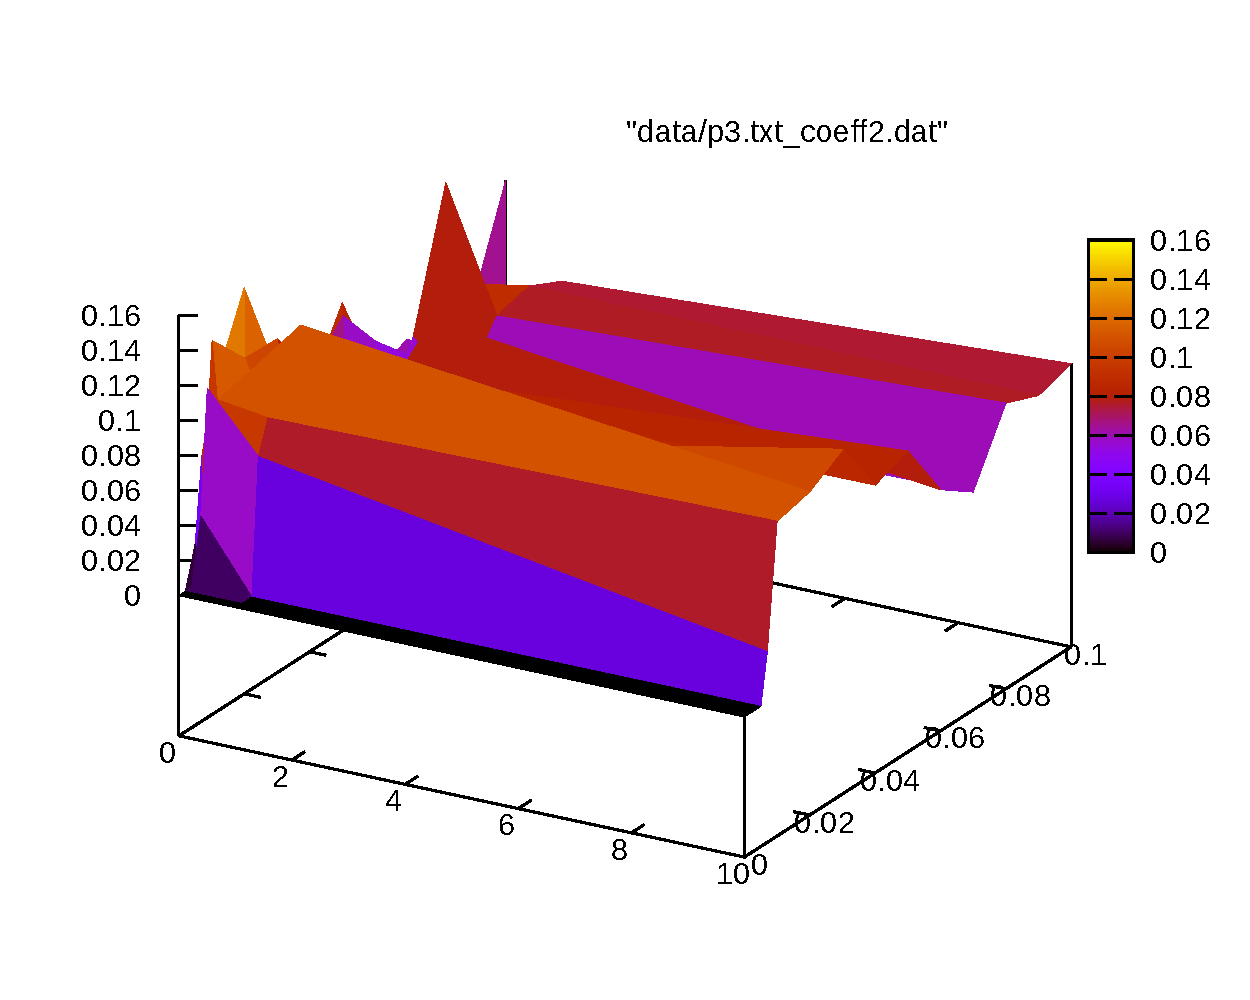
\includegraphics[scale=0.25]{figs/even/p3.txt_coeff2.dat.pdf}
  \end{tabular}
  \caption{Поверхности дисперсии для формулы \eqref{eq:res_0}.}
  \label{tabl:res_even}
\end{table}

Из графиков видно, что от шума, накладываемого на значения длины волны, дисперсия значений
первого и второго коэффициентов практически не зависит. В то же время дисперсия значений
первого коэффициента зависит от дисперсии шума коэффициента преломления практически линейно,
тогда как для второго коэффициента после некоторого характерного значения зависимость теряется.
Кроме того, дисперсия третьего коэффициента формулы не имеет явной гладкой зависимости от
дисперсии шума длины волны или коэффициента преломления, что еще раз подтверждает его достаточно
случайную природу.

Физическая интерпретация этих результатов~--- при построении прибора для измерения дисперсии
сред значительное внимание следует уделять точности измерения коэффициента преломления,
тогда как измерения длины волны могут быть неточны вплоть до нескольких процентов. Кроме того,
предложенный метод прямо указывает, на каких интервалах шума какой будет выигрыш в точности
предсказания от небольшого увеличения точности.

Отметим так же, что для коэффициентов, стоящих на одних и тех же местах, графики дисперсии
похожи даже для разных веществ. Из этого можно сделать вывод, что полученная формула
действительно описывает наблюдаемое физическое явление~--- именно такая зависимость и
<<должна>> была бы получиться, и что полученная зависимость носит универсальный характер,
не являясь переобученной моделью.

Кроме того, значения дисперсии не превосходят настоящие значения параметров по порядку величины,
что означает, в частности, что вещества могут быть различены даже не очень точным рефрактометром.

\paragraph{Стабильность некорректного решения.}

Аналогично исследуем стабильность решения \eqref{eq:res_incorrect}. Для данных значений дисперсии
приведем только графики зависимости, см. таблицу \ref{tabl:res_incorrect}.

\begin{table}[h]
  \centering
  \begin{tabular}{c c c}
	Материал 1 & Материал 2 & Материал 3 \\ \hline
	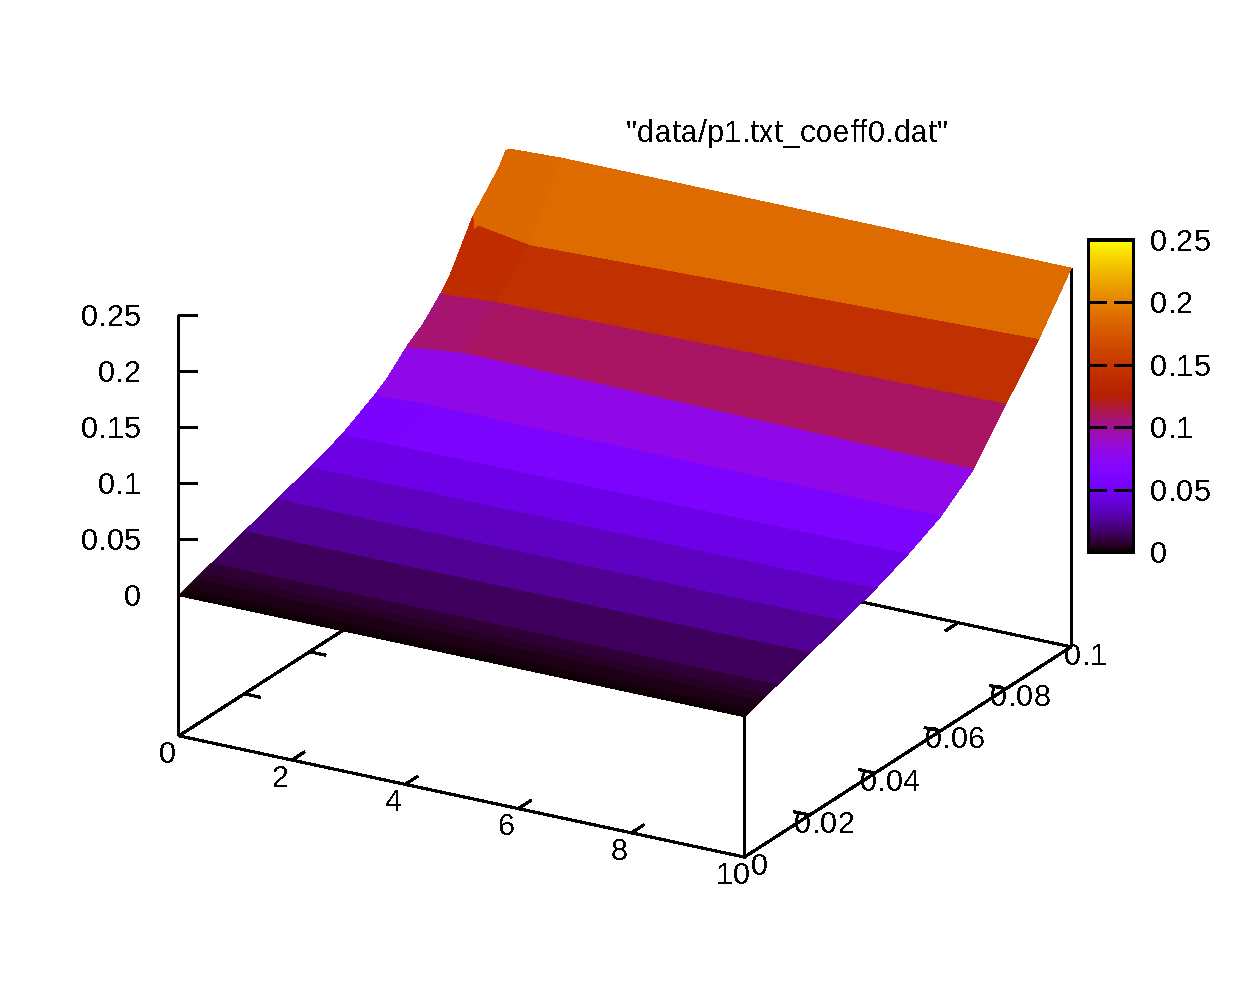
\includegraphics[scale=0.20]{figs/all/p1.txt_coeff0.dat.pdf} & 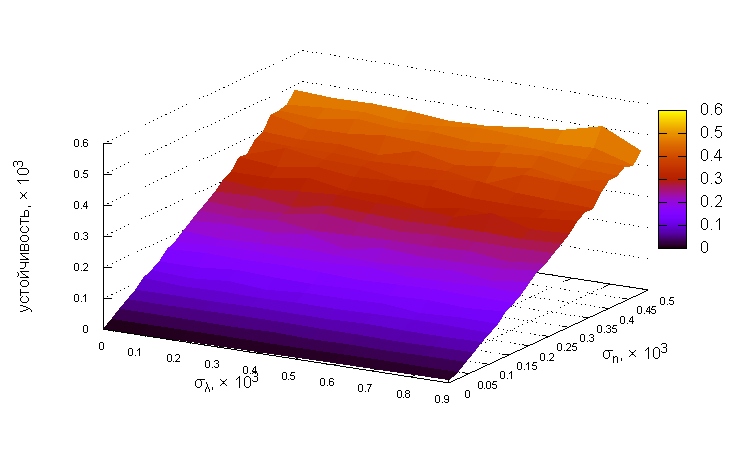
\includegraphics[scale=0.20]{figs/all/p2.txt_coeff0.dat.pdf} & 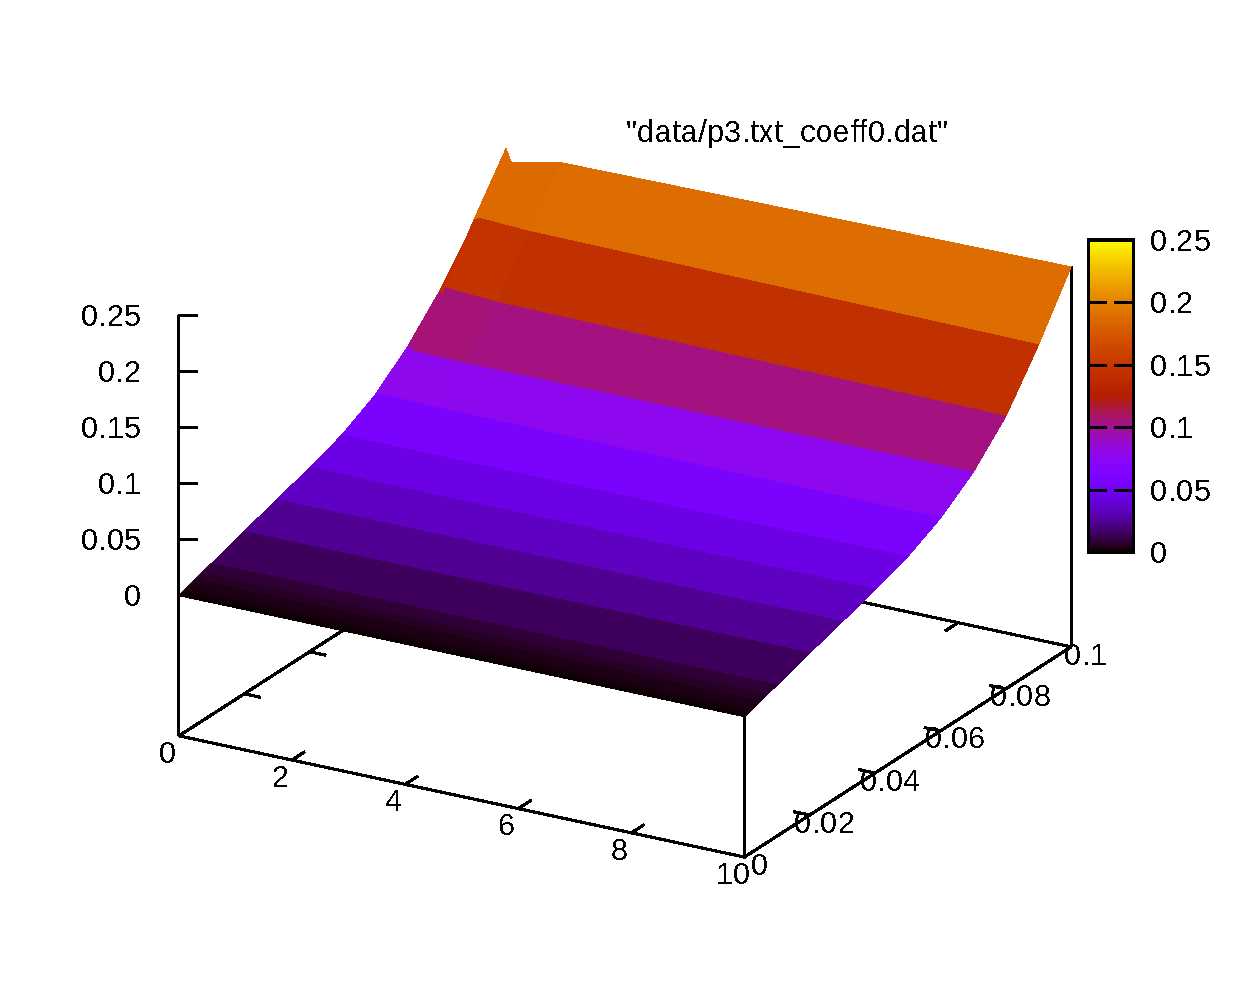
\includegraphics[scale=0.20]{figs/all/p3.txt_coeff0.dat.pdf} \\
	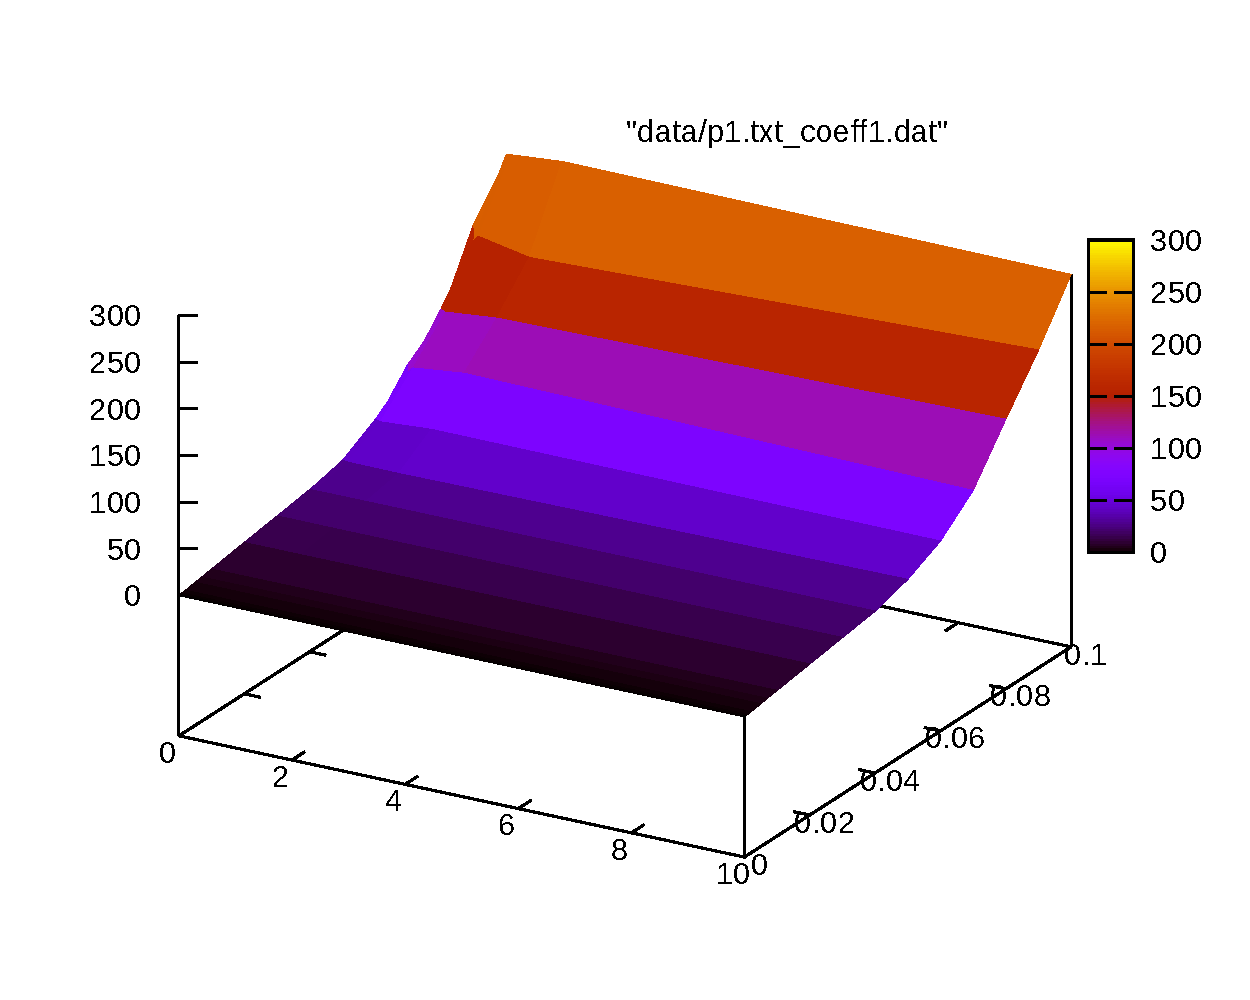
\includegraphics[scale=0.20]{figs/all/p1.txt_coeff1.dat.pdf} & 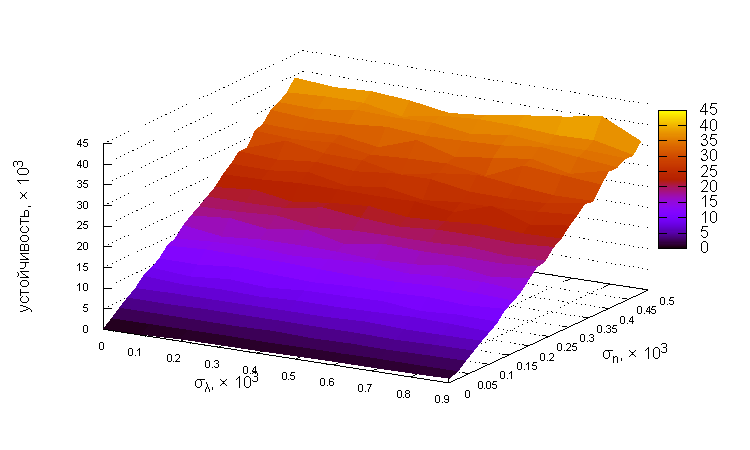
\includegraphics[scale=0.20]{figs/all/p2.txt_coeff1.dat.pdf} & 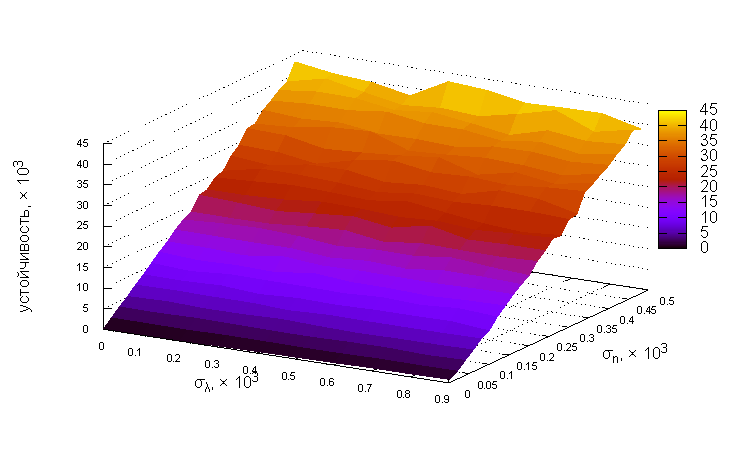
\includegraphics[scale=0.20]{figs/all/p3.txt_coeff1.dat.pdf} \\
	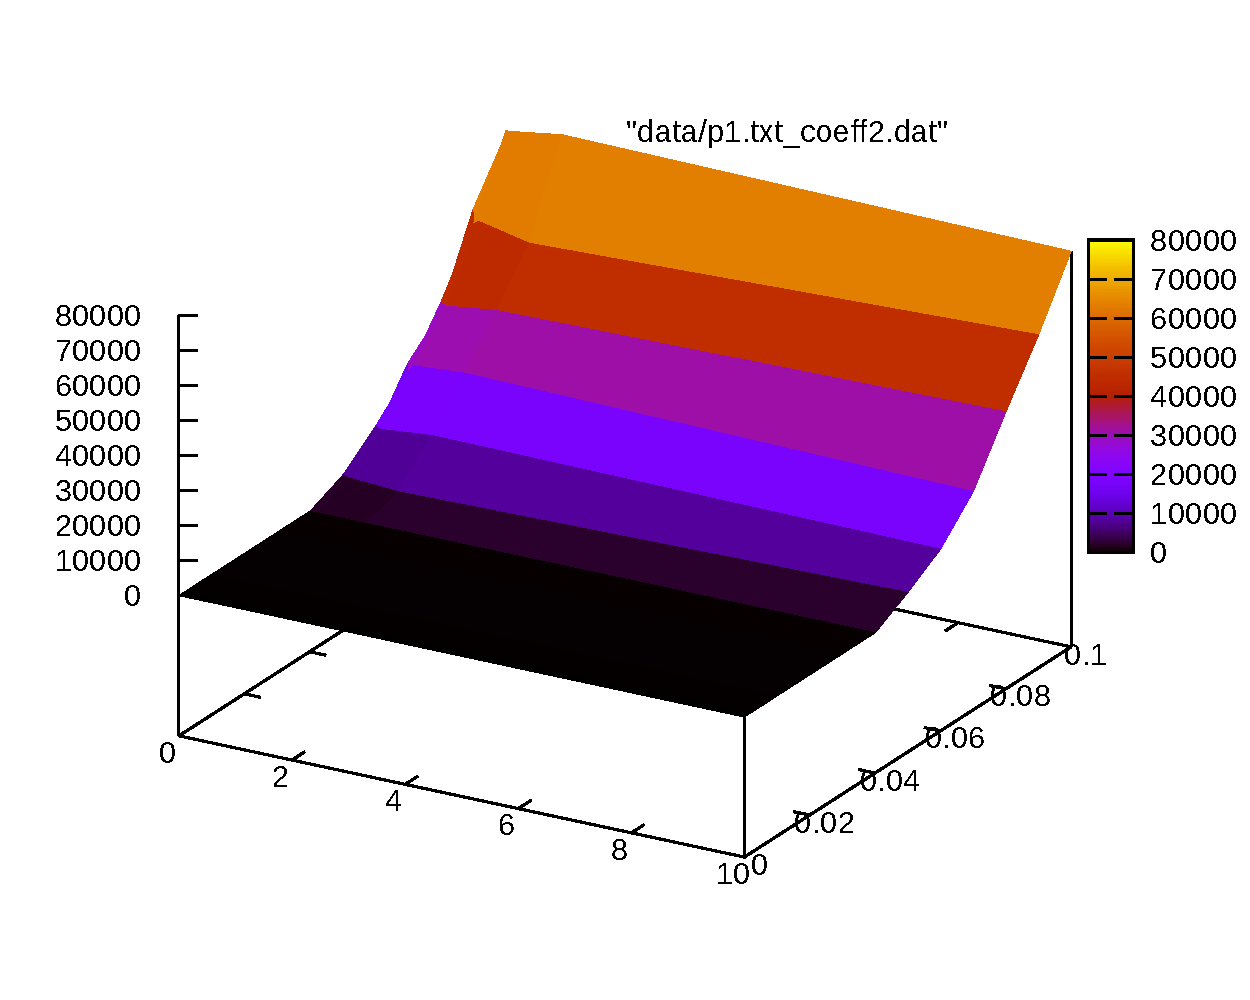
\includegraphics[scale=0.20]{figs/all/p1.txt_coeff2.dat.pdf} & 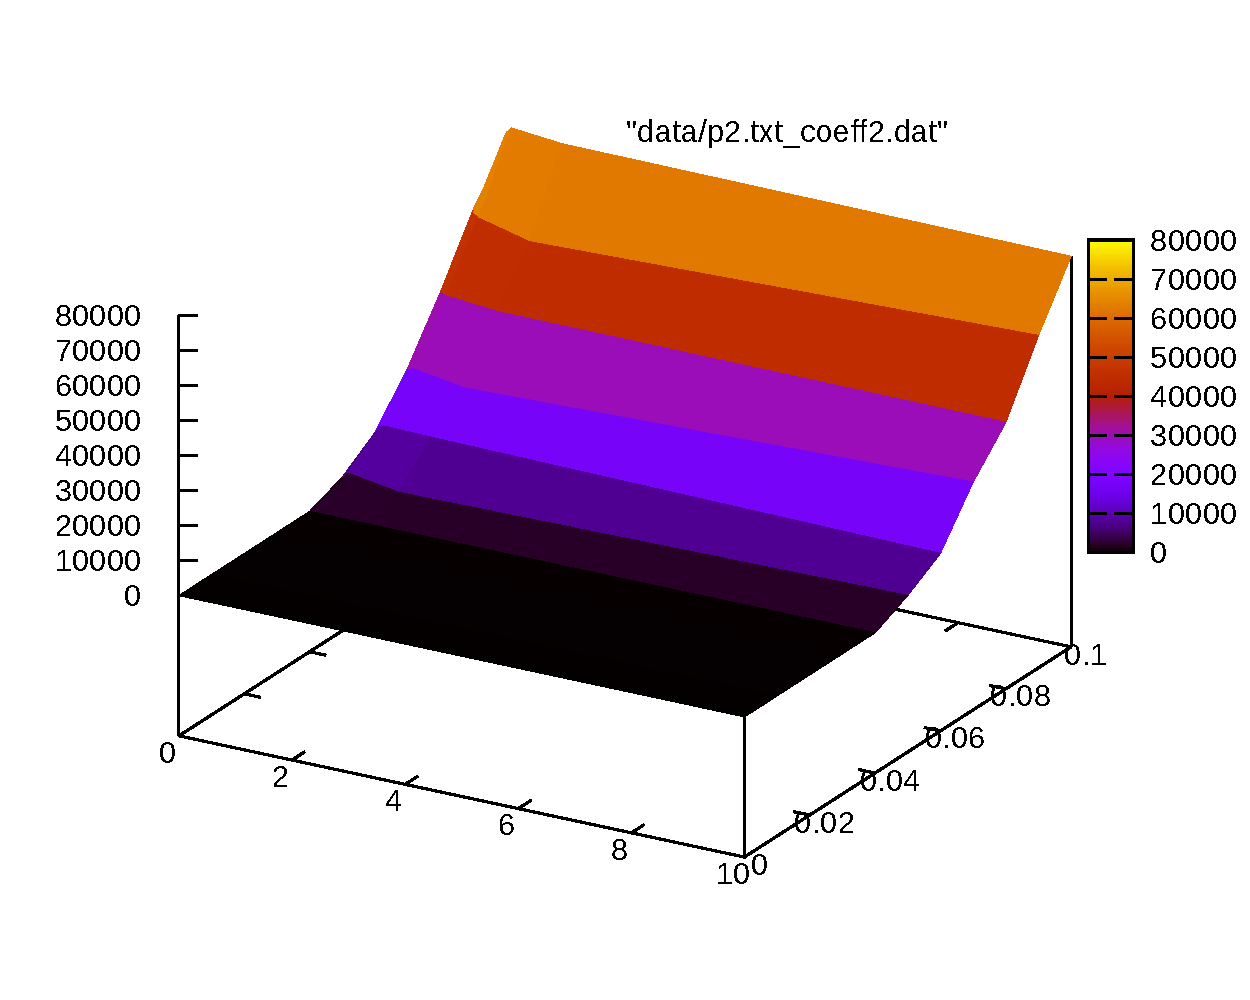
\includegraphics[scale=0.20]{figs/all/p2.txt_coeff2.dat.pdf} & 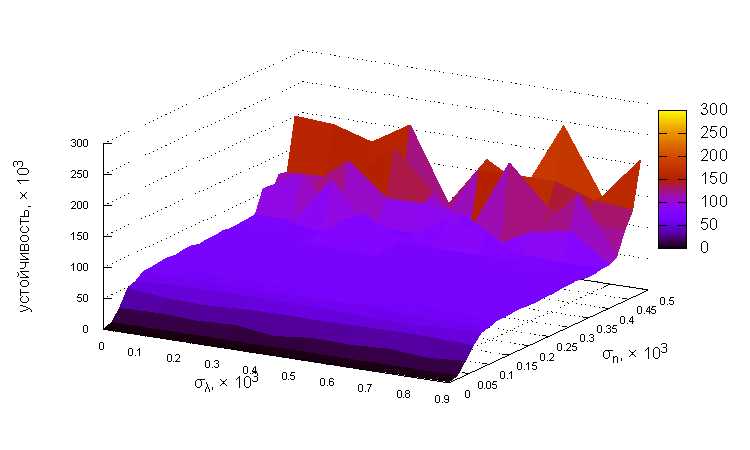
\includegraphics[scale=0.20]{figs/all/p3.txt_coeff2.dat.pdf} \\
	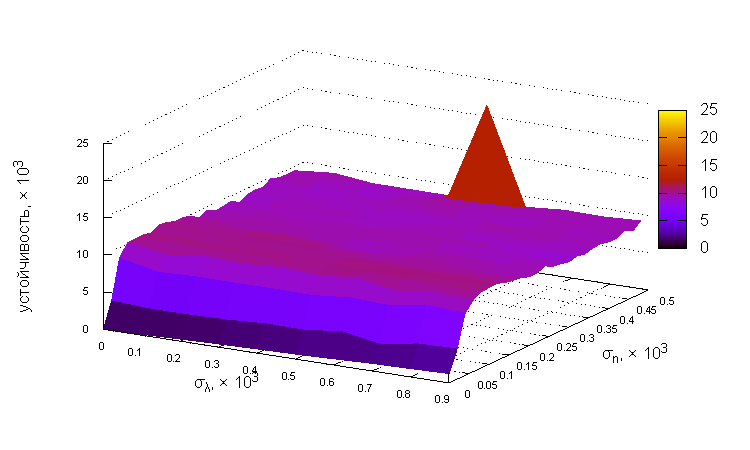
\includegraphics[scale=0.20]{figs/all/p1.txt_coeff3.dat.pdf} & 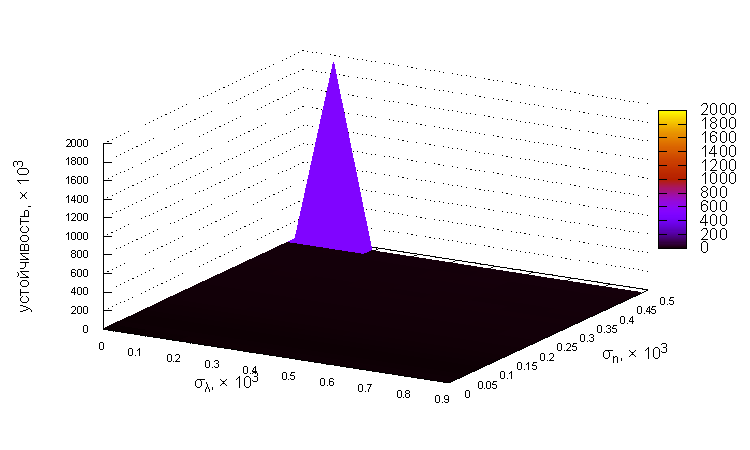
\includegraphics[scale=0.20]{figs/all/p2.txt_coeff3.dat.pdf} & 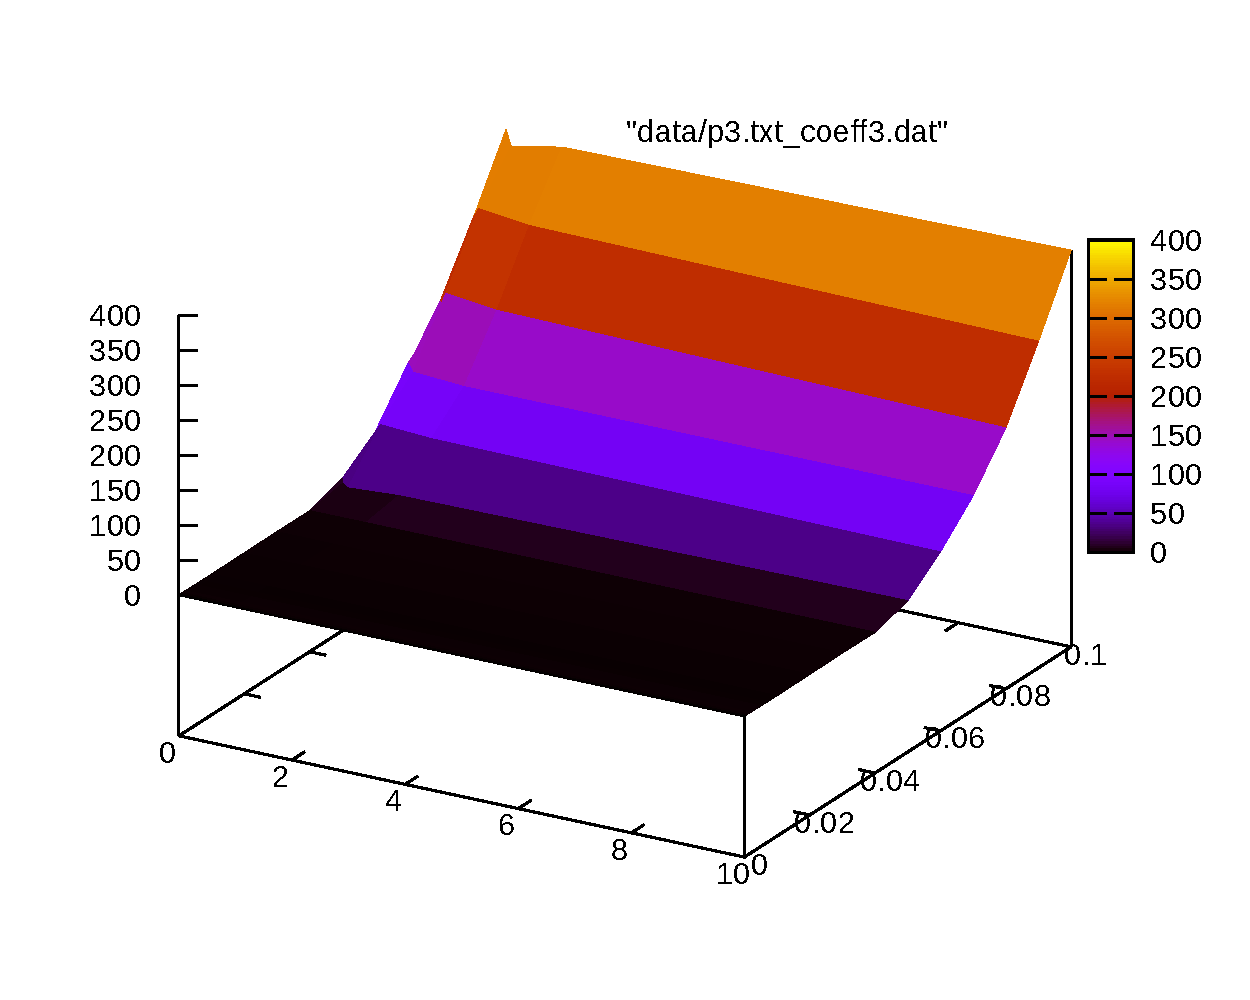
\includegraphics[scale=0.20]{figs/all/p3.txt_coeff3.dat.pdf} \\
	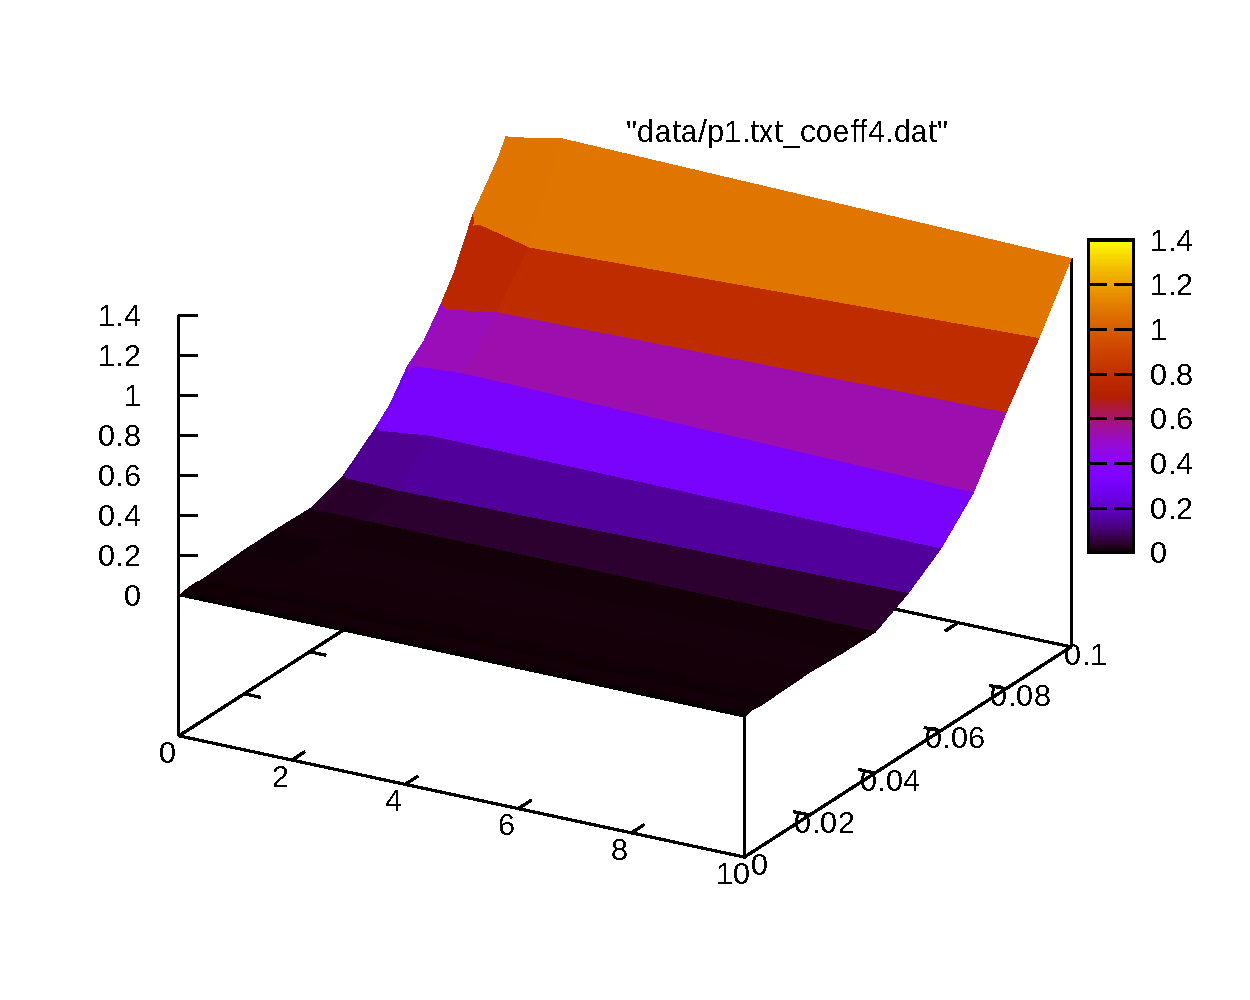
\includegraphics[scale=0.20]{figs/all/p1.txt_coeff4.dat.pdf} & 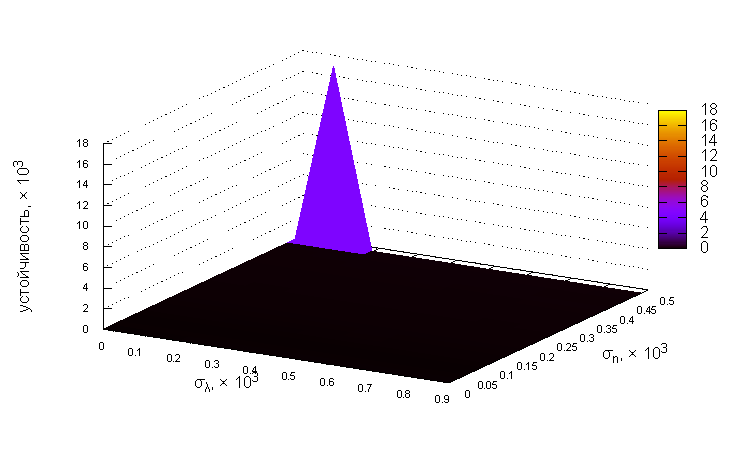
\includegraphics[scale=0.20]{figs/all/p2.txt_coeff4.dat.pdf} & 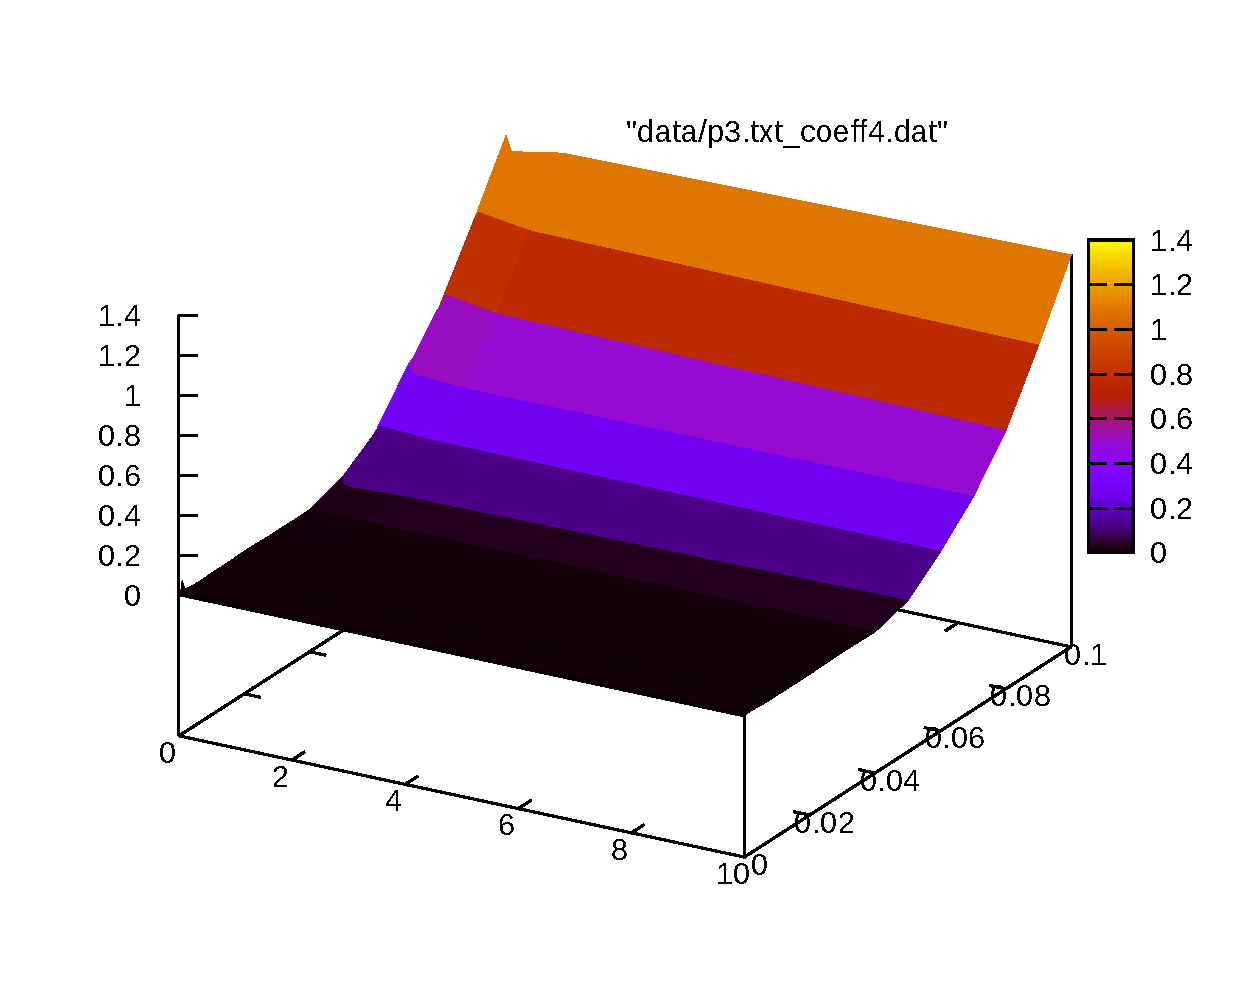
\includegraphics[scale=0.20]{figs/all/p3.txt_coeff4.dat.pdf} \\
	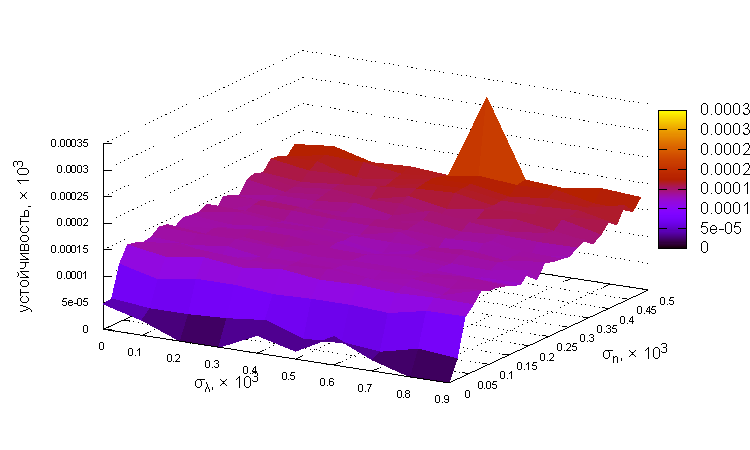
\includegraphics[scale=0.20]{figs/all/p1.txt_coeff5.dat.pdf} & 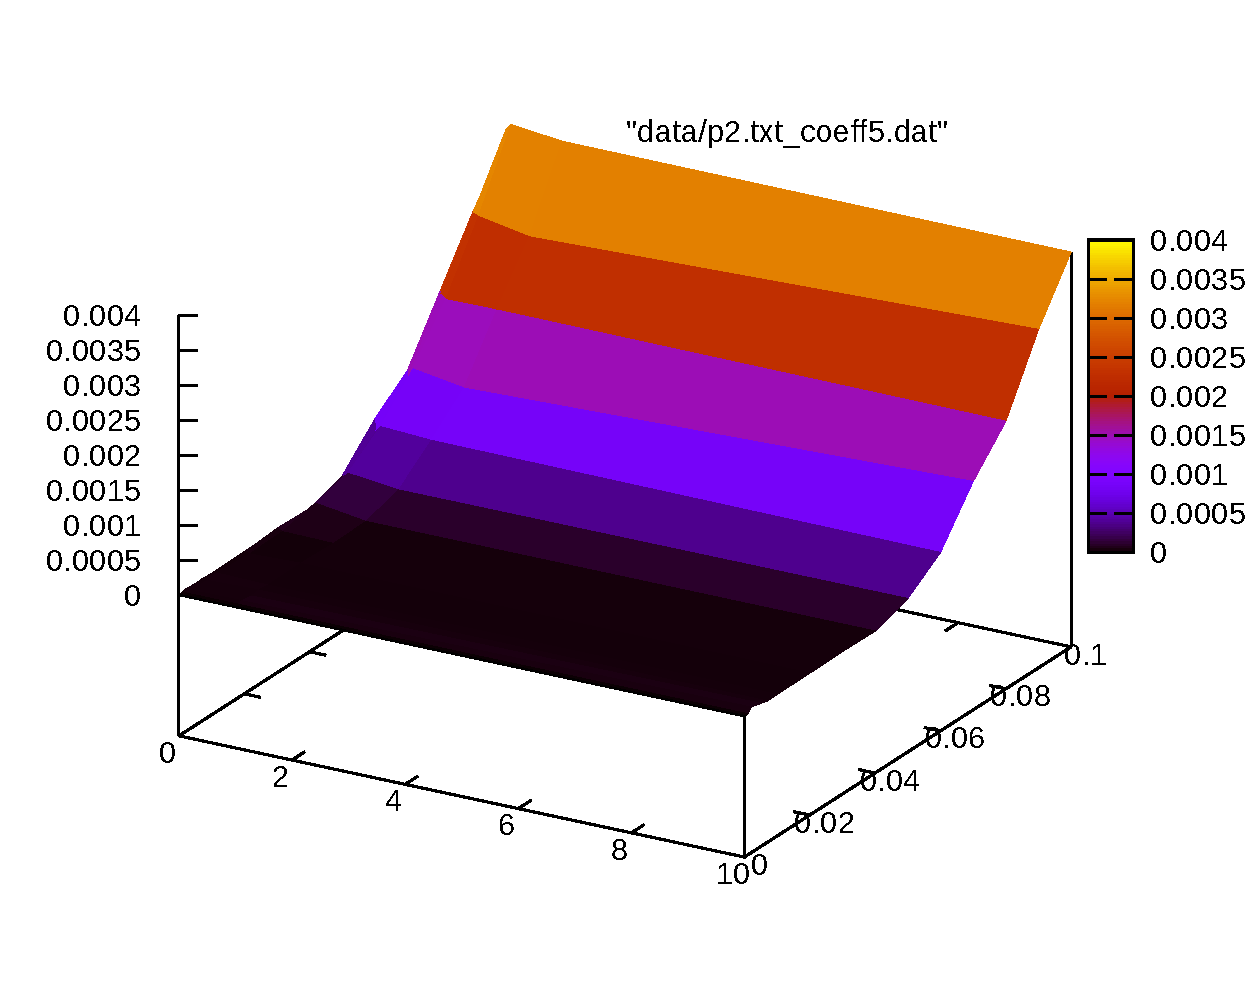
\includegraphics[scale=0.20]{figs/all/p2.txt_coeff5.dat.pdf} & 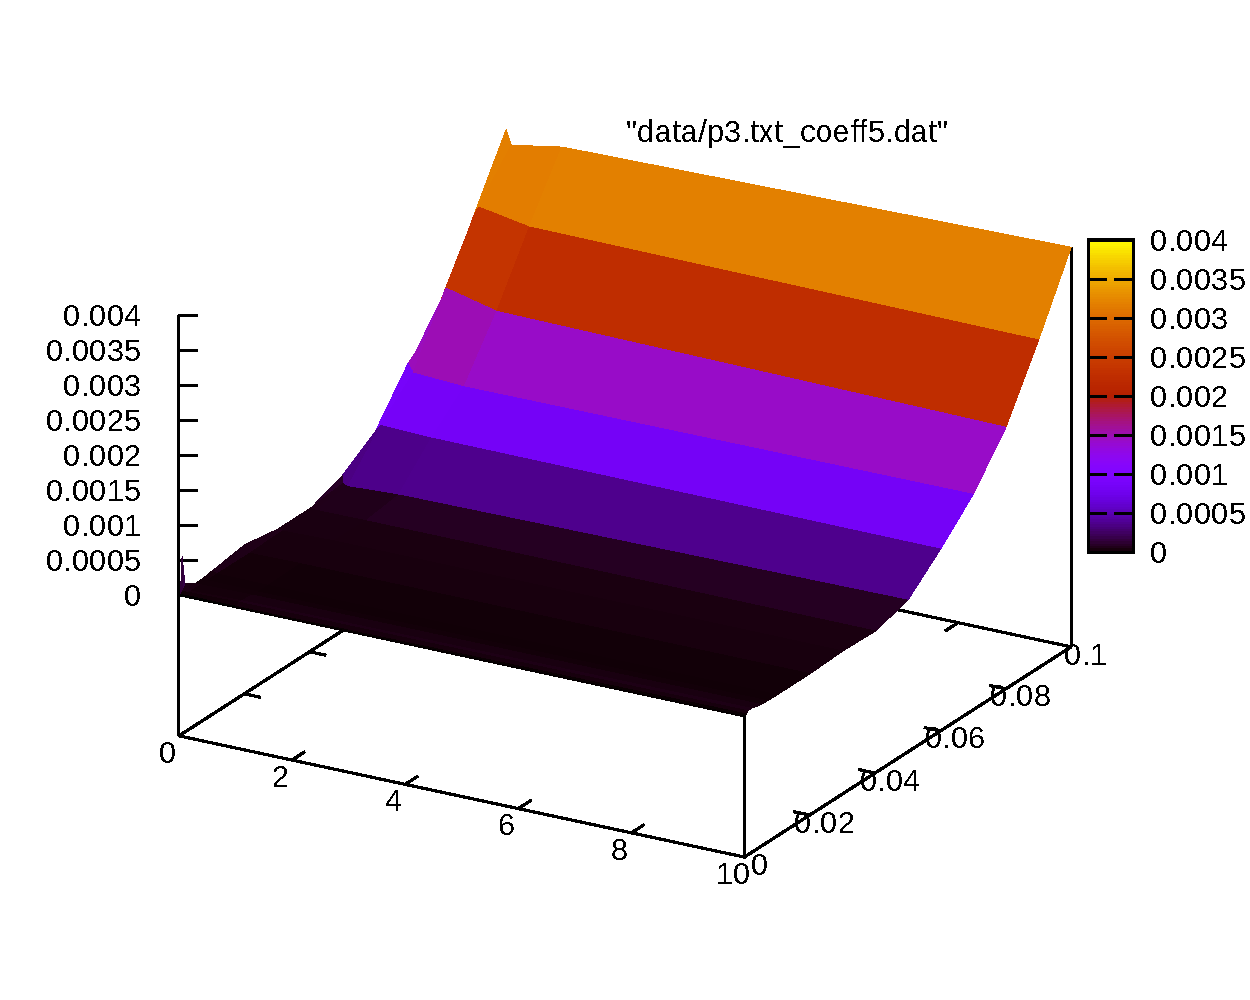
\includegraphics[scale=0.20]{figs/all/p3.txt_coeff5.dat.pdf}
  \end{tabular}
  \caption{Поверхности дисперсии для формулы \eqref{eq:res_incorrect}.}
  \label{tabl:res_incorrect}
\end{table}

Из графиков видно, что в случае формулы \eqref{eq:res_incorrect} дисперсия соответствующих
параметров существенно превышает таковую для \eqref{eq:res_0}. В частности, второй, третий
и четвертый коэффициенты имеют дисперсию, на порядки превышающую характерные значения самих
коэффициентов.

Данные результаты свидетельствуют о переобучении, и что полученная модель не может быть
использована для надежного приближения экспериментальных данных ввиду большой чувствительности
к шумам.

\FloatBarrier

\paragraph{Исследование экспертного предположения.}

Экспертом предположено, что формула так же может иметь вид
\begin{equation}
  n(\lambda) = a + \frac{b}{c - \frac{1}{\lambda^2}},
  \label{eq:resonance}
\end{equation}
если измерения находятся вблизи точки резонанса.

Результаты нахождения параметров $a, b$ и $c$ методом Левенберга-Марквардта
приведены в таблице \ref{tabl:resonance_coeffs}.

\begin{table}[h]
  \centering
  \begin{tabular}{| c | r | r | r |} \hline
	Материал	& $a$		& $b$					& $c$					\\ \hline
	1			& 1.385		& $1.79 \cdot 10^{-7}$	& $-4.49 \cdot 10^{-6}$	\\ \hline
	2			& 1.372		& $1.62 \cdot 10^{-7}$	& $-4.59 \cdot 10^{-6}$	\\ \hline
	3			& 1.361		& $1.21 \cdot 10^{-7}$	& $-3.75 \cdot 10^{-6}$	\\ \hline
  \end{tabular}
  \caption{Значения коэффициентов формулы \eqref{eq:resonance}.}
  \label{tabl:resonance_coeffs}
\end{table}

Коэффициент $c$ в формуле \eqref{eq:resonance} имеет смысл резонансной
частоты, приближение к которой описывается этой формулой, поэтому коэффициент
$c$ должен быть неотрицательным. Ввиду этого полученные результаты не
имеют физического смысла.

\begin{table}[h]
  \centering
  \begin{tabular}{c c c}
	Материал 1 & Материал 2 & Материал 3 \\ \hline
	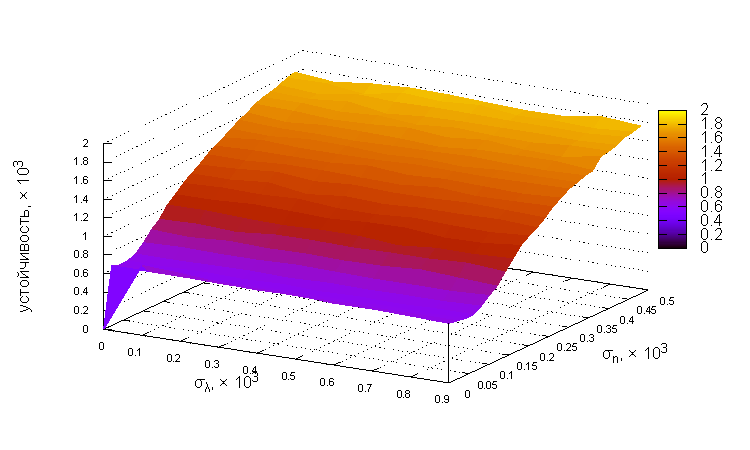
\includegraphics[scale=0.25]{figs/resonance/p1.txt_coeff0.dat.pdf} & 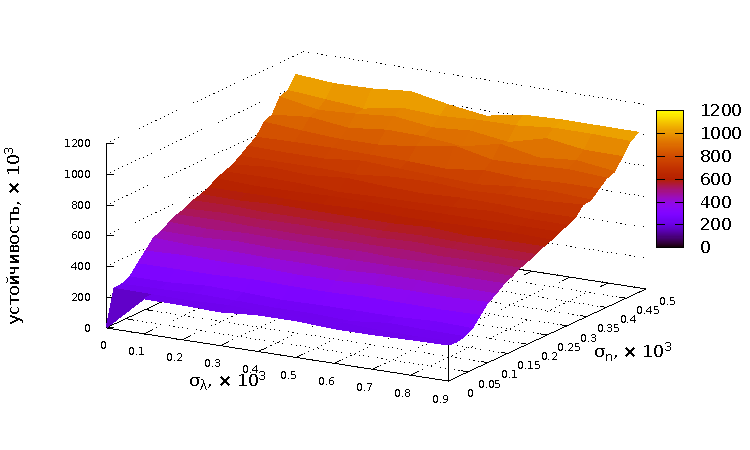
\includegraphics[scale=0.25]{figs/resonance/p2.txt_coeff0.dat.pdf} & 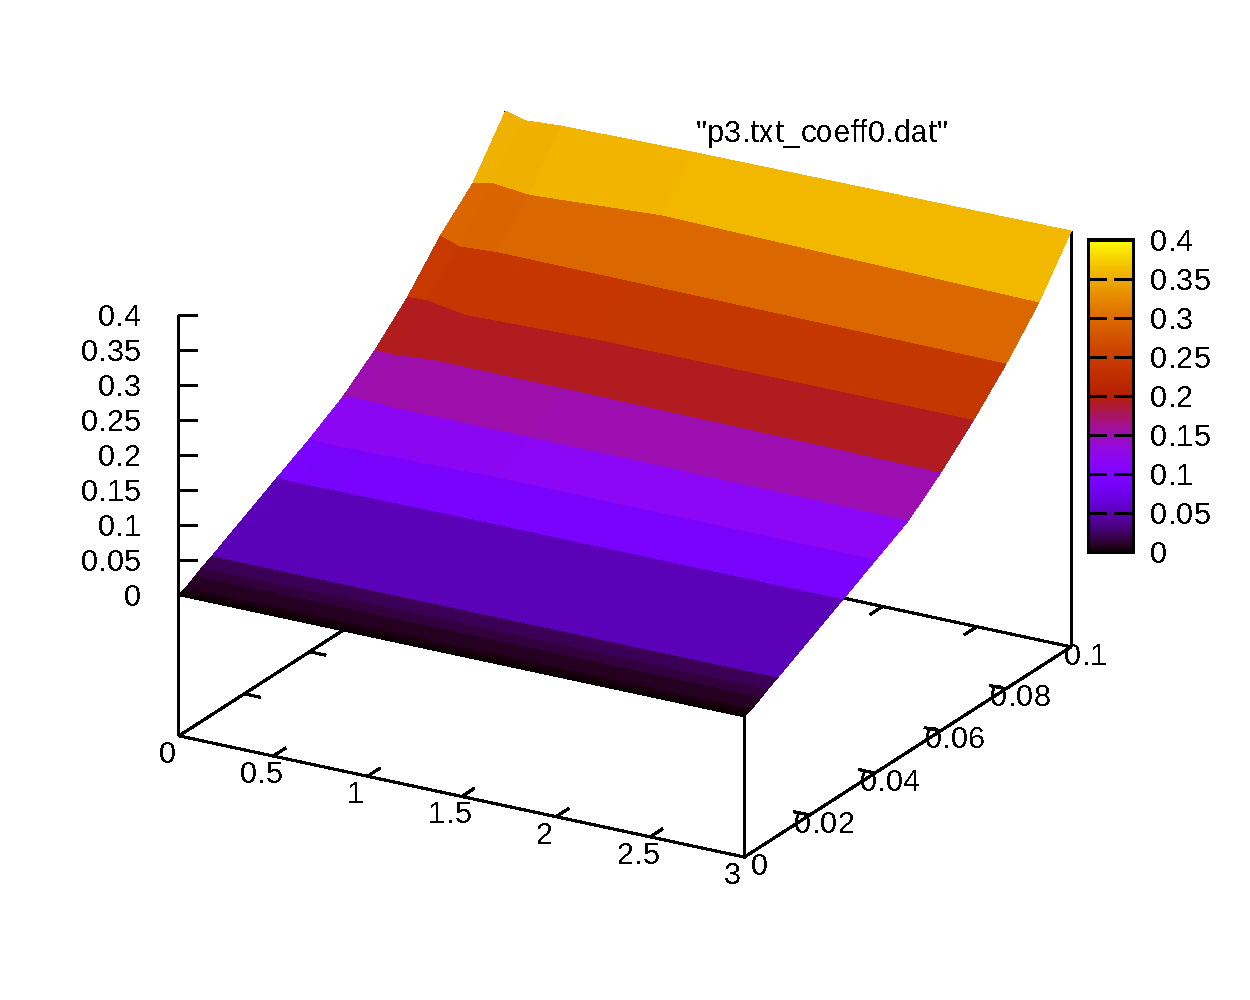
\includegraphics[scale=0.25]{figs/resonance/p3.txt_coeff0.dat.pdf} \\
	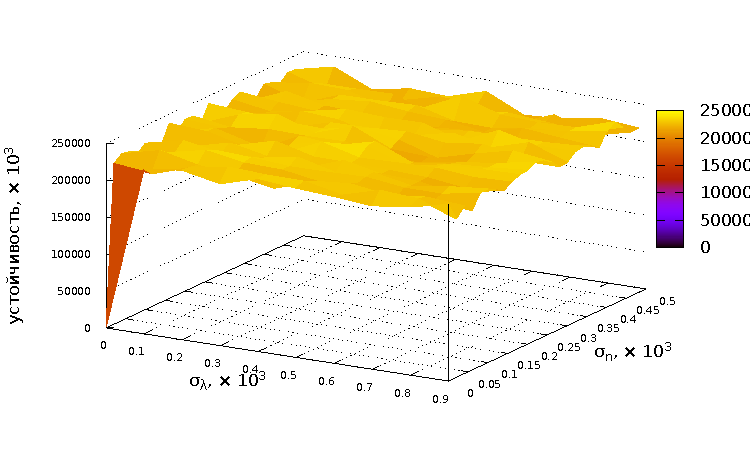
\includegraphics[scale=0.25]{figs/resonance/p1.txt_coeff1.dat.pdf} & 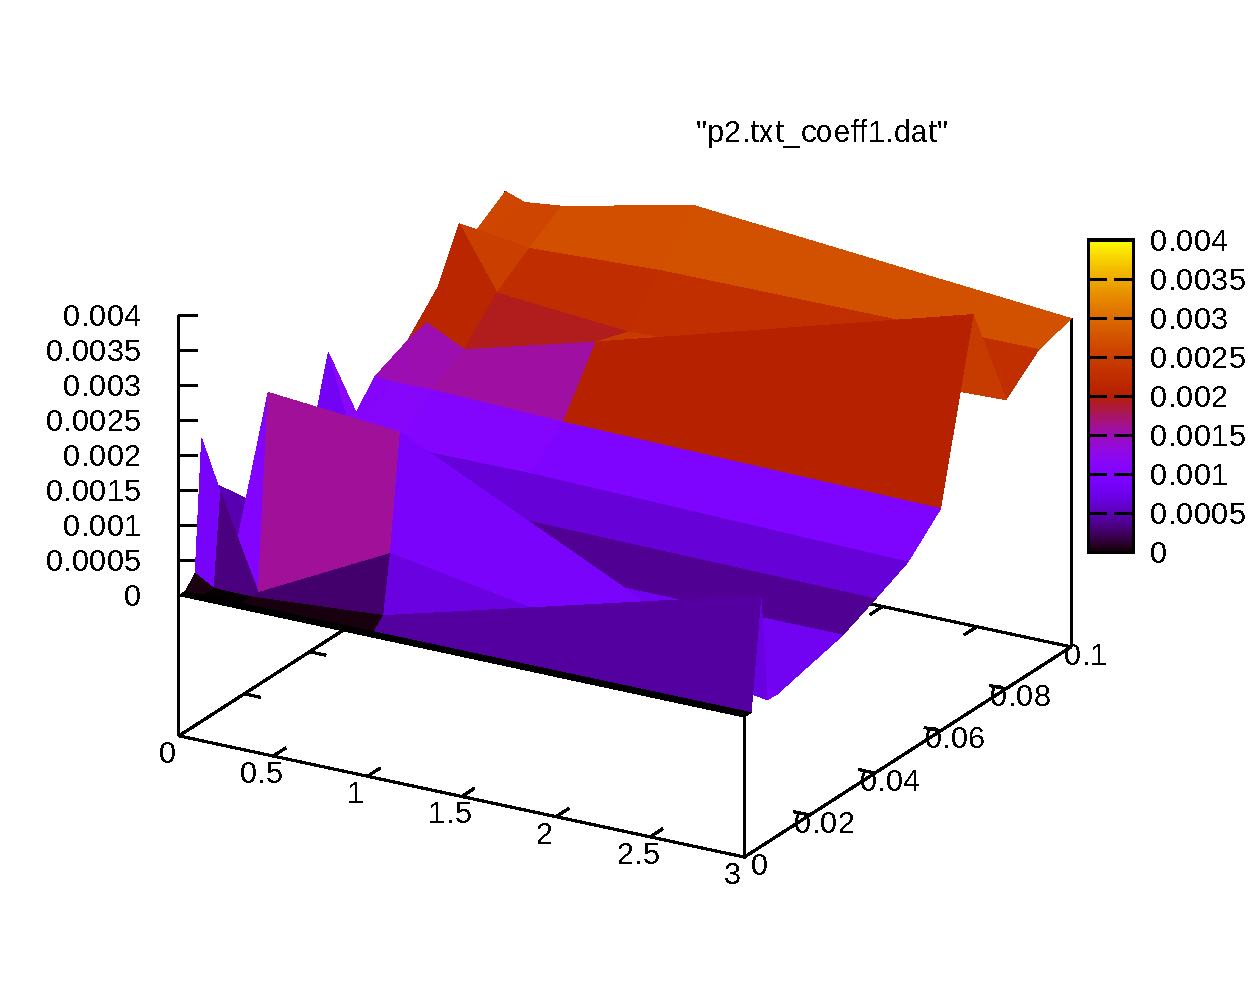
\includegraphics[scale=0.25]{figs/resonance/p2.txt_coeff1.dat.pdf} & 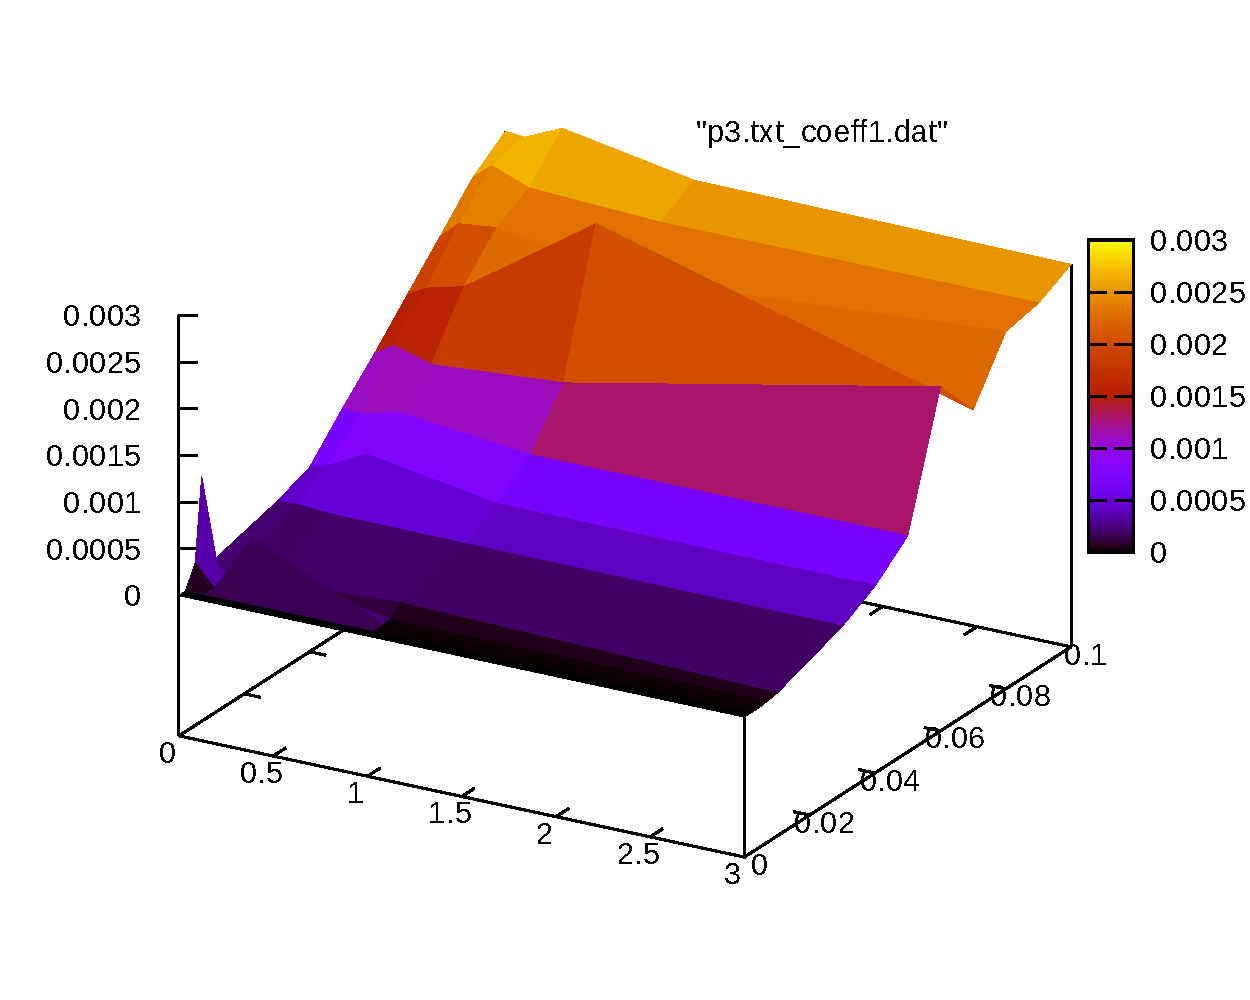
\includegraphics[scale=0.25]{figs/resonance/p3.txt_coeff1.dat.pdf} \\
	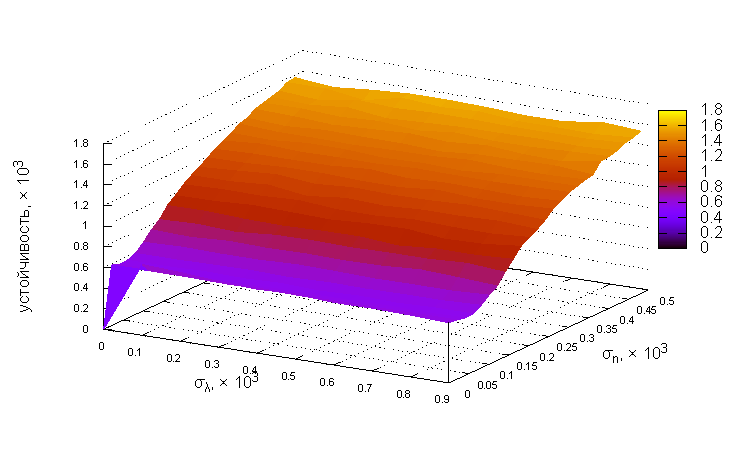
\includegraphics[scale=0.25]{figs/resonance/p1.txt_coeff2.dat.pdf} & 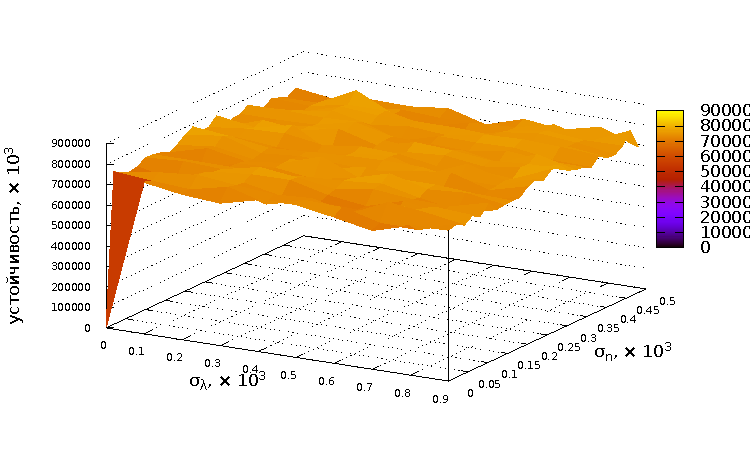
\includegraphics[scale=0.25]{figs/resonance/p2.txt_coeff2.dat.pdf} & 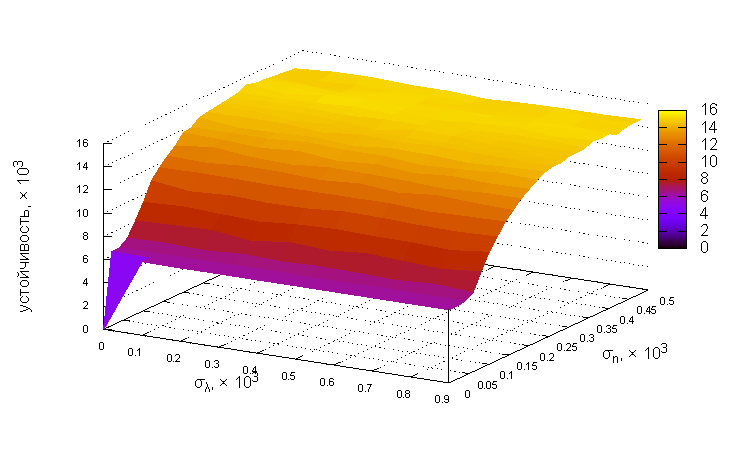
\includegraphics[scale=0.25]{figs/resonance/p3.txt_coeff2.dat.pdf}
  \end{tabular}
  \caption{Поверхности дисперсии для формулы \eqref{eq:resonance}.}
  \label{tabl:res_resonance}
\end{table}

Тем не менее, исследуем стабильность данного решения тем же методом, что и в
предыдущих случаях. Поверхности дисперсии приведены в таблице \ref{tabl:res_resonance}.

Отметим, что характерная дисперсия первого коэффициента на порядок больше, чем
для формулы \eqref{eq:res_0}, что затрудняет различение веществ в смеси при
достаточно большой погрешности измерения $\lambda$, однако дисперсии второго и
третьего коэффициента примерно на порядок меньше, чем для формулы
\eqref{eq:res_0}.

Поверхности дисперсии также не являются настолько же гладкими, как для формулы
\eqref{eq:res_0}.

Все это позволяет заключить, что, хотя экспериментальные данные хорошо
описываются формулой \eqref{eq:resonance}, они не являются корректными с
экспертно-физической точки зрения. Это, в частности, подтверждается экспертным
соображением об ограничениях на коэффициенты формулы \eqref{eq:resonance},
которые не выполняются в полученной модели.

\section{Заключение}

Предложенный в \cite{Rudoy13} алгоритм позволяет получить интерпретируемую аналитическую
формулу, описывающую зависимость коэффициента преломления среды от длины волны.
Введенный штраф за сложность позволяет избежать переобучения без прибегания к методам
вроде скользящего контроля, и таким образом отпадает необходимость в контрольной выборке.

Хотя другие алгоритмы, такие как SVM-регрессия, могут демонстрировать более высокое
качество приближения данных, их результаты неинтерпретируемы и не защищены от переобучения
<<по построению>>, поэтому требуют разделения выборки на обучающую и контрольную. Кроме
того, их структурные параметры так же требуют оценки по методам вроде кросс-валидации.

Предложенный в настоящей работе метод оценки стабильности решения позволяет исследовать вклад различных
членов результирующей суперпозиции в решение, и зависимость изменения этих членов от
случайных шумов во входных данных. В частности, в прикладных областях данный метод позволяет
выявить, какие именно элементы признакового описания объектов в генеральной совокупности
наиболее чувствительны к шуму. Кроме того, для корректных с экспертной точки зрения
решений оказывается, что они стабильны, в то время как некорректные результаты нестабильны.

\FloatBarrier

\bibliographystyle{babunsrt-lf}
%\bibliographystyle{babunsrt}
%\bibliographystyle{unsrt}
\bibliography{bibliography}

\end{document}
